% Credit Risk Intelligence Platform - final project report (FAST-NUCES, MLOps, Semester 7)
% Build:  latexmk -pdf -interaction=nonstopmode main.tex   (see report/README.md)
\documentclass[11pt,a4paper]{article}

\usepackage[utf8]{inputenc}
\usepackage[T1]{fontenc}
\usepackage{lmodern}
\usepackage[margin=2.3cm,headheight=14pt]{geometry}
\usepackage{microtype}
\usepackage{graphicx}
\usepackage{xcolor}
\usepackage{booktabs}
\usepackage{longtable}
\usepackage{tabularx}
\usepackage{array}
\usepackage{multirow}
\usepackage{amsmath}
\usepackage{caption}
\usepackage{subcaption}
\usepackage{placeins}
\usepackage{enumitem}
\usepackage{fancyhdr}
\usepackage{titlesec}
\usepackage{listings}
\usepackage{needspace}
\usepackage{etoolbox}
\usepackage[hidelinks]{hyperref}

\graphicspath{{../docs/evidence/}{../docs/diagrams/}{../reports/plots/}{../reports/}}

% ---------- blue and white theme (matches the web UI) ----------
\definecolor{navy}{HTML}{0A2159}
\definecolor{blue}{HTML}{1D5BDB}
\definecolor{paleblue}{HTML}{EEF4FF}
\definecolor{ruleblue}{HTML}{DDE5F2}
\titleformat{\section}{\Large\bfseries\color{navy}}{\thesection}{0.7em}{}[{\color{blue}\titlerule[0.8pt]}]
\titleformat{\subsection}{\large\bfseries\color{navy}}{\thesubsection}{0.7em}{}
\titleformat{\subsubsection}{\normalsize\bfseries\color{blue}}{\thesubsubsection}{0.7em}{}
\hypersetup{colorlinks=false,pdfborder={0 0 0}}
\captionsetup{font=small,labelfont={bf,color=navy},labelsep=period}
\setlist{itemsep=2pt,topsep=4pt}
\setlength{\parindent}{0pt}
\setlength{\emergencystretch}{3em}
\setlength{\parskip}{5pt}
\renewcommand{\arraystretch}{1.18}

\pagestyle{fancy}
\fancyhf{}
\fancyhead[L]{\small\color{navy}Credit Risk Intelligence Platform}
\fancyhead[R]{\small\color{navy}MLOps Final Report}
\fancyfoot[C]{\small\thepage}
\renewcommand{\headrulewidth}{0.4pt}
\renewcommand{\headrule}{\hbox to\headwidth{\color{ruleblue}\leaders\hrule height \headrulewidth\hfill}}

\lstset{basicstyle=\ttfamily\footnotesize,breaklines=true,frame=single,rulecolor=\color{ruleblue},
  backgroundcolor=\color{paleblue},columns=fullflexible,keepspaces=true,showstringspaces=false,
  xleftmargin=2pt,xrightmargin=2pt}

\pretocmd{\section}{\Needspace*{9\baselineskip}}{}{}
\pretocmd{\subsection}{\Needspace*{6\baselineskip}}{}{}
\newcommand{\code}[1]{\texttt{\detokenize{#1}}}
\newcommand{\simd}{{\bfseries SIMULATED}}
\newcommand{\status}[1]{\textbf{\color{blue}#1}}
\newcolumntype{L}[1]{>{\raggedright\arraybackslash}p{#1}}
\newcolumntype{R}{>{\raggedleft\arraybackslash}X}
\newcommand{\hdr}[1]{\textbf{\color{navy}#1}}

\begin{document}

% =====================================================================================================
\begin{titlepage}
\thispagestyle{empty}
\begin{center}
\vspace*{1.2cm}
{\color{blue}\rule{\linewidth}{2pt}}\\[1.2cm]
{\Huge\bfseries\color{navy} Credit Risk Intelligence Platform}\\[0.5cm]
{\Large An end-to-end MLOps system for credit-card default risk:\\ data versioning, orchestration, serving, AWS delivery,\\ Kubernetes, monitoring and retraining}\\[1.4cm]
{\color{blue}\rule{0.5\linewidth}{1pt}}\\[1.0cm]
{\large\bfseries Final project report}\\[0.3cm]
FAST-NUCES \quad|\quad MLOps \quad|\quad Semester 7\\[1.6cm]
{\large\bfseries Group 14}\\[0.3cm]
\begin{tabular}{ll}
\toprule
\hdr{Name} & \hdr{Roll number}\\
\midrule
Hashir Rauf & 23L-2572\\
Junaid Minhas & 23L-2559\\
Ahsan Ijaz & 23L-2617\\
\bottomrule
\end{tabular}\\[1.2cm]
{\normalsize Repository: \url{https://github.com/Hashir-Rauf/Credit-Risk-Intelligence-Platform}}\\[0.3cm]
{\normalsize 27 November 2026}\\[1.5cm]
\fcolorbox{ruleblue}{paleblue}{\parbox{0.85\linewidth}{\small
\textbf{Not a lending tool.} This is a university course project. The model ranks customers by modelled risk; its score is \emph{not} a calibrated probability of default and must not be used for real credit decisions.}}
\end{center}
\end{titlepage}

\tableofcontents
\clearpage

% =====================================================================================================
\section{Summary and status}
\label{sec:summary}

The project predicts whether a credit-card customer will default in the next month (UCI \emph{Default of Credit Card Clients}, 30\,000 customers, 22.1\,\% positive). The engineering goal is everything around the model: versioned data, reproducible training, a quality gate that blocks bad models, a serving path with rollback, observability, and a retraining loop that never promotes a model on its own.

\textbf{Headline results.}
\begin{itemize}
\item \textbf{Model:} random forest, held-out test ROC-AUC \textbf{0.7883}, PR-AUC 0.578, KS 0.440, recall 0.600 and precision 0.509 at threshold 0.5 (Section~\ref{sec:model}). The quality gate (ROC-AUC $\geq$ 0.77) passed.
\item \textbf{Delivery:} a green CI pipeline, a manually approved CD pipeline using GitHub OIDC (no stored AWS keys), and a deployment on AWS ECS Fargate that serves predictions and the web UI (Section~\ref{sec:aws}).
\item \textbf{Operations:} Kubernetes scaling and self-healing demonstrated, three alert families fired and resolved on purpose, and a drift-triggered retrain whose challenger was correctly \emph{rejected} (Sections~\ref{sec:k8s} and~\ref{sec:monitoring}).
\item \textbf{Security:} gitleaks over the whole history, bandit, pip-audit and Trivy are clean; least-privilege IAM; 11 project risks assessed (Section~\ref{sec:security}).
\end{itemize}

\textbf{Honest status at the time of writing.} Items that were \emph{not} demonstrated are listed here and again where they matter; nothing below should be read as claiming them.

\begin{table}[htbp]
\centering\small
\begin{tabularx}{\linewidth}{L{5.2cm}L{2.4cm}X}
\toprule
\hdr{Item} & \hdr{Status} & \hdr{Note}\\
\midrule
Data, DVC, modelling, CI, serving, orchestration & done & evidence in Sections~\ref{sec:data}--\ref{sec:pipelines}\\
AWS deployment (API + web UI) & done & ECS Fargate, task definition rev.\ 5, deployed by the CD workflow\\
AWS rollback run & done & Rollback workflow moved the service from revision 6 to 5 and the smoke test passed\\
AWS alarm firing & done & 5xx alarm set to ALARM by a manual state change (not by a real error), history and screenshot captured\\
AWS cost screenshot & done & Cost Explorer, 20--26 November, daily by service: total -\$0.00 (covered by credits)\\
AWS teardown with leftover check & \status{pending} & runs last, after the demonstration\\
Promotion of a better challenger & \status{unit-tested only} & the live retrain reproduced the champion exactly, so no better model existed\\
Kubernetes autoscaler (HPA) under load & \status{not run} & manifest passes a server-side dry run only\\
Drift, delayed labels & \simd{} & resampled held-out rows with shifted features; always labelled\\
Reproduction by someone other than the author & \status{pending} & required exit criterion of the last phase\\
\bottomrule
\end{tabularx}
\caption{Status of the deliverables.}
\end{table}

% =====================================================================================================
\section{Architecture}
\label{sec:arch}

\begin{figure}[htbp]
\centering
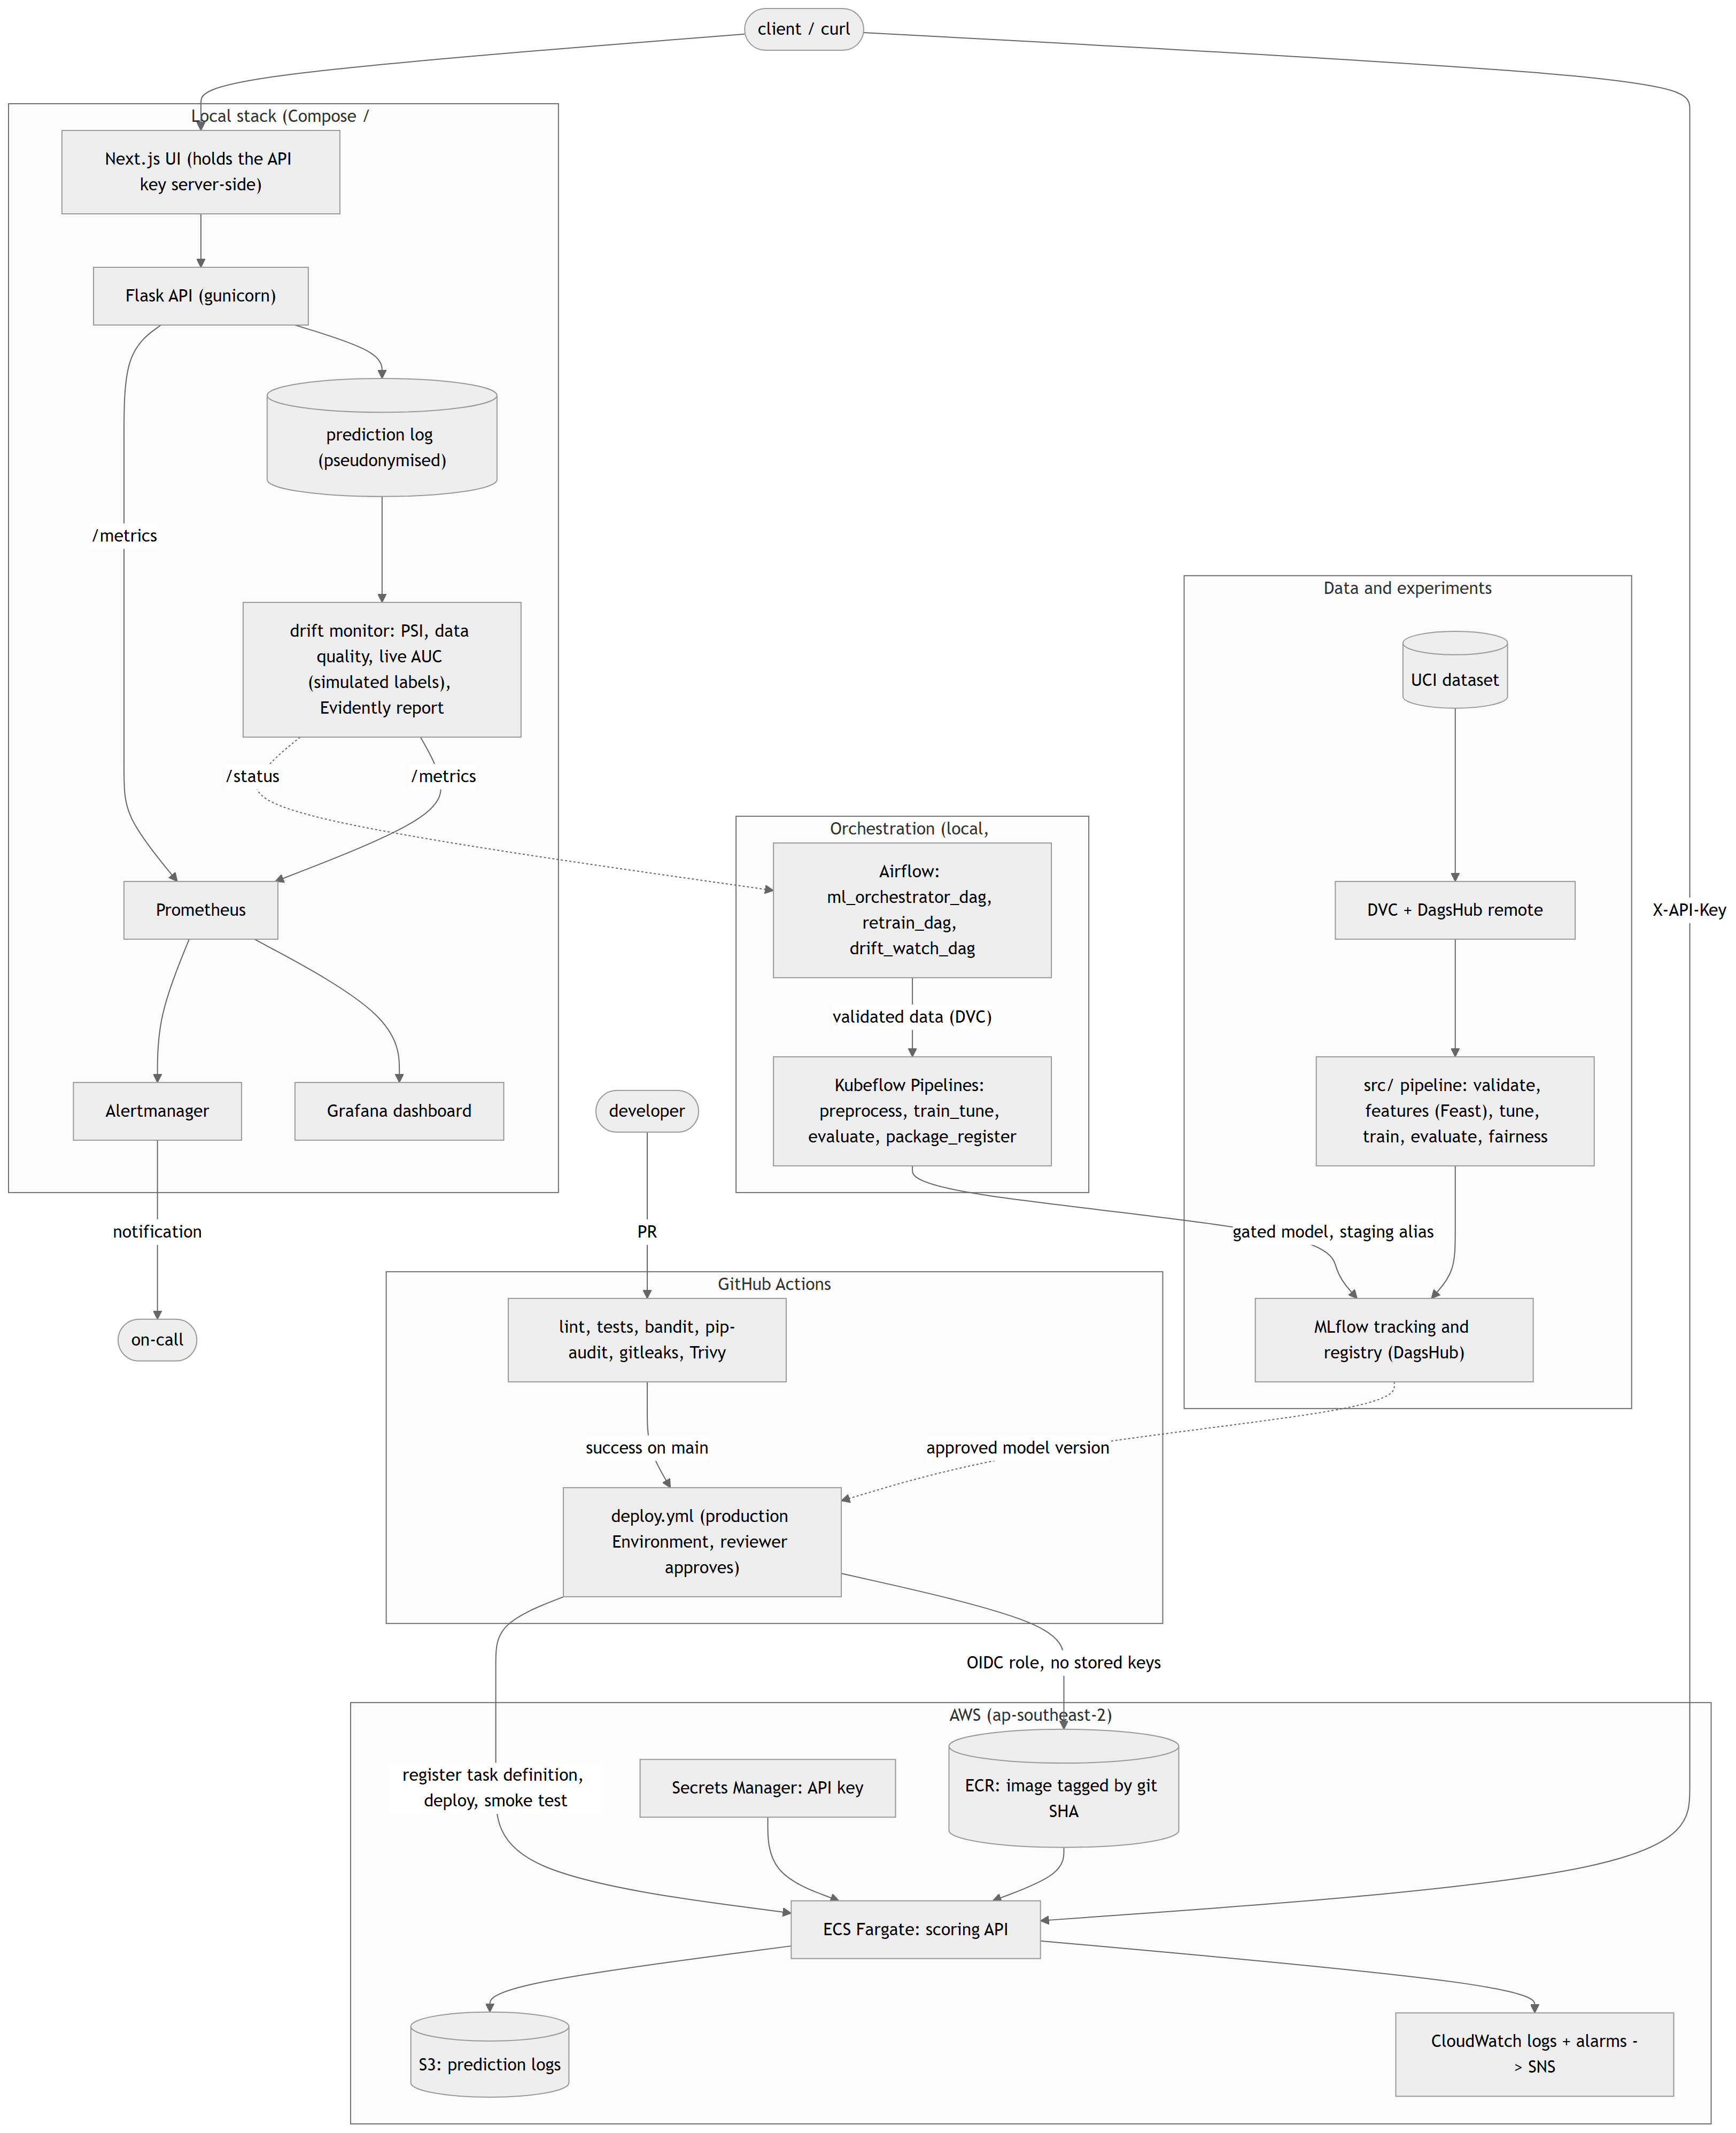
\includegraphics[width=\linewidth,height=0.78\textheight,keepaspectratio]{architecture.png}
\caption{System architecture: data and experiments, orchestration, serving, delivery and operations.}
\end{figure}

\begin{description}[leftmargin=3.2cm,style=nextline]
\item[Data and experiments] DVC versions data and models (S3 and DagsHub remotes); MLflow on DagsHub tracks runs and holds the model registry (\code{credit-risk-default-model}, aliases \code{champion}, \code{staging}, \code{challenger}); Feast supplies features.
\item[Orchestration] Airflow triggers one run; Kubeflow Pipelines on Minikube executes preprocess $\rightarrow$ train/tune $\rightarrow$ evaluate $\rightarrow$ package/register with a quality-gate branch.
\item[Serving] Flask under gunicorn with API-key authentication, schema-generated validation and Prometheus metrics; a Next.js UI that keeps the key server-side; a BentoML packaging of the same model.
\item[Delivery] GitHub Actions: CI (lint, tests, scanners, image scan) and CD (build, scan, push to ECR by git SHA, ECS deploy, smoke test, rollback) with a manual approval environment and OIDC instead of stored keys.
\item[Operations] Prometheus, Grafana, Alertmanager; a pseudonymised prediction log; a drift monitor (PSI, data quality, live AUC from replayed labels, Evidently report); a retrain DAG and a promotion/rollback procedure.
\end{description}

\begin{figure}[htbp]
\centering
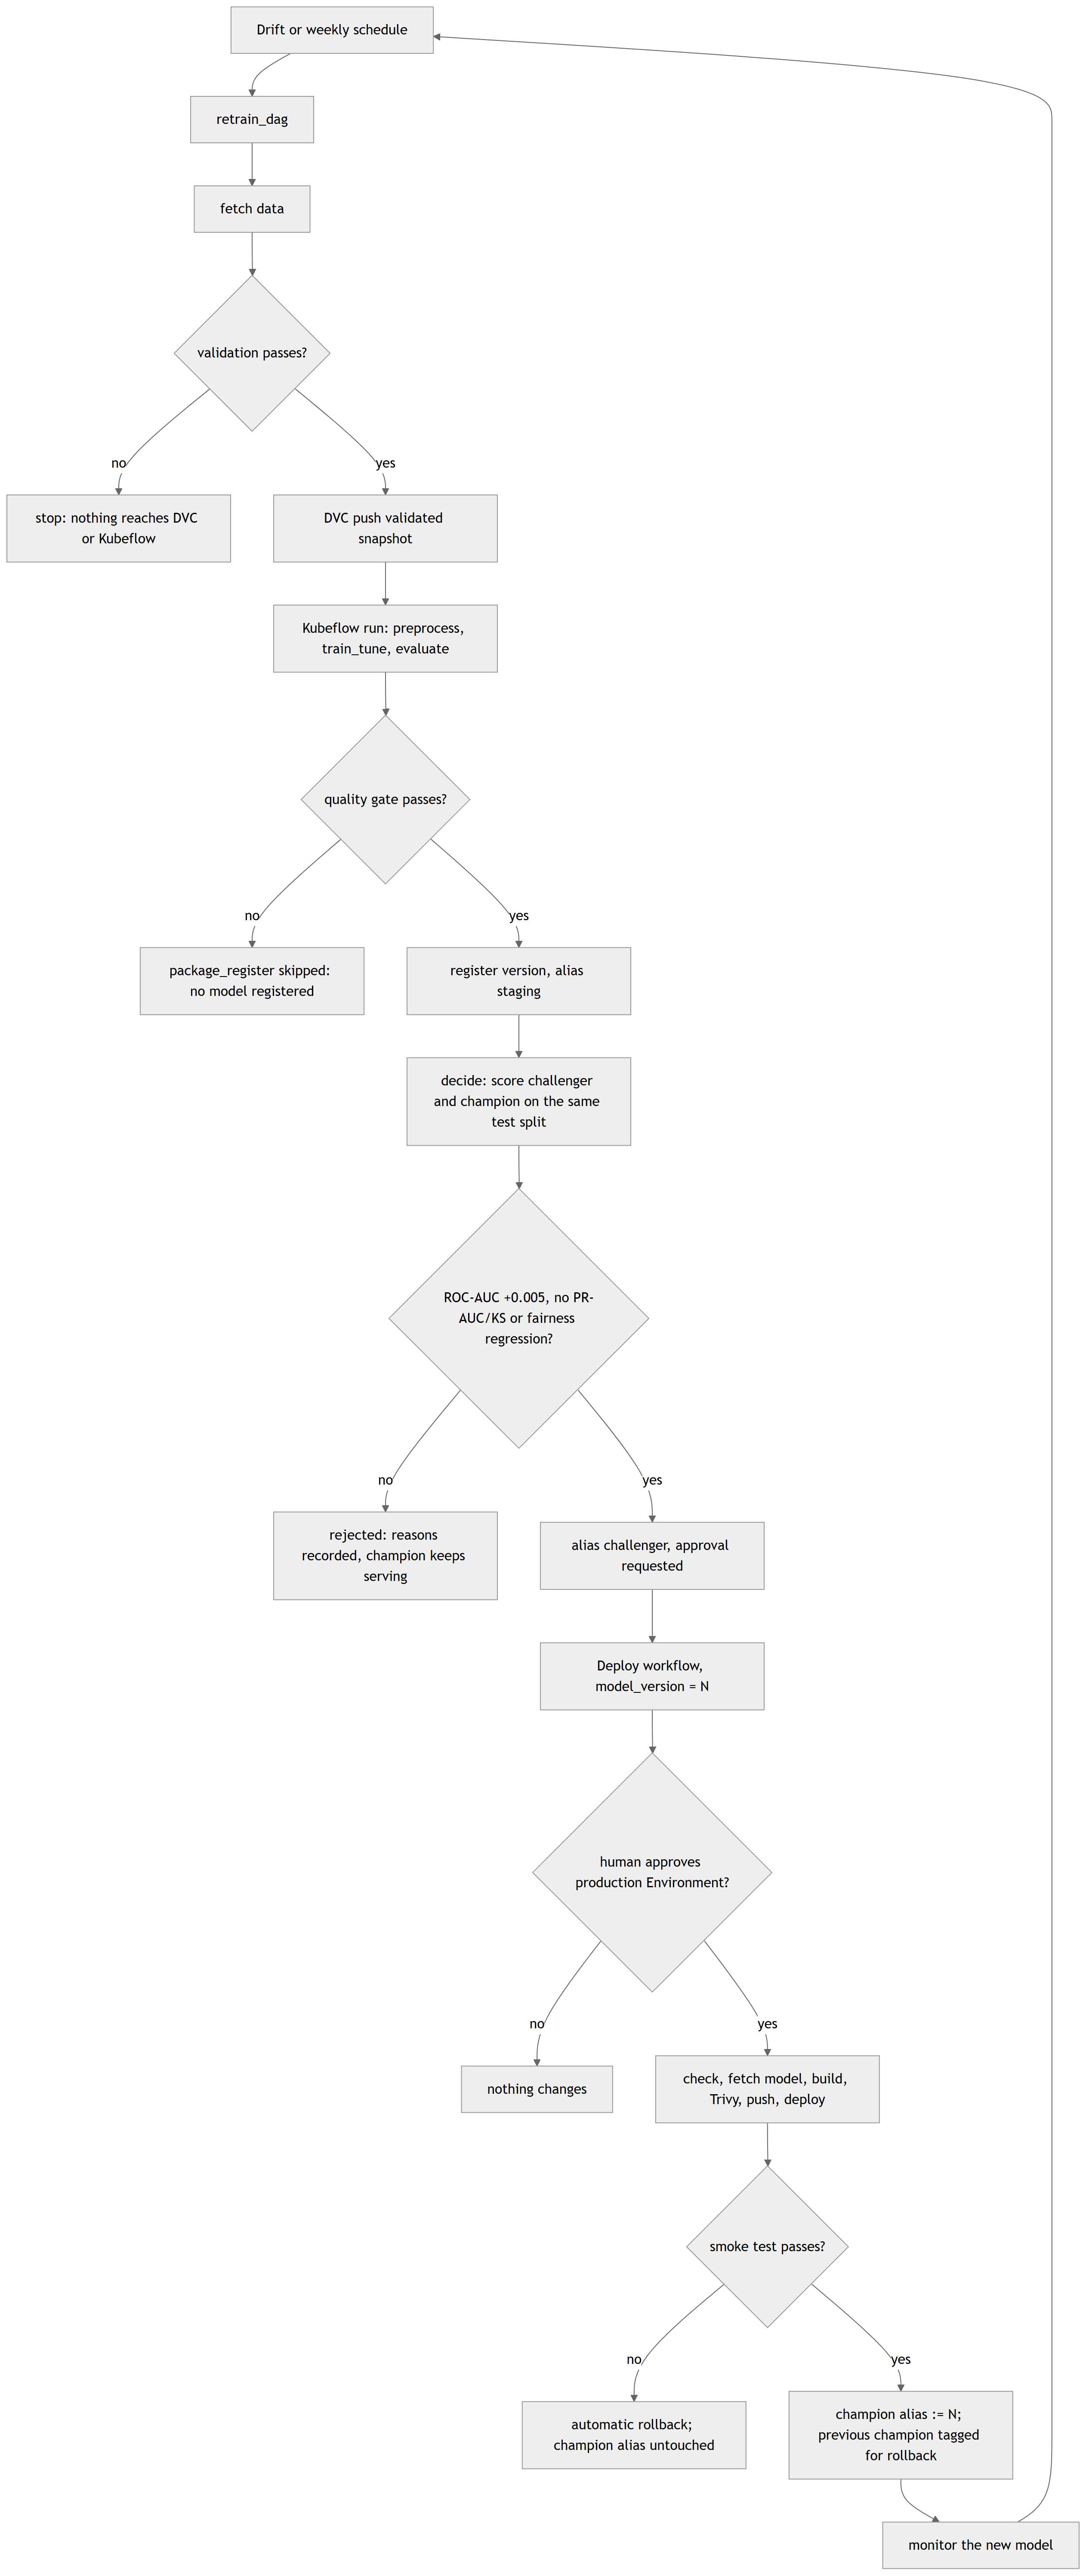
\includegraphics[width=\linewidth,height=0.78\textheight,keepaspectratio]{workflow.png}
\caption{Retrain and promotion workflow. The retrain DAG recommends; only the approved Deploy workflow moves the \code{champion} alias, and only after a smoke-tested deployment.}
\end{figure}

\subsection{Key design decisions}
\begin{longtable}{L{3.9cm}L{5.2cm}L{4.7cm}}
\toprule
\hdr{Decision} & \hdr{Why} & \hdr{Trade-off}\\
\midrule\endhead
Random forest champion chosen from three tuned families & best validation ROC-AUC among simple models (Table~\ref{tab:families}) & scores are uncalibrated, so the API returns \code{risk_score}, never a probability\\
Sensitive attributes excluded from the inputs & fairness rule; an ablation shows using them adds nothing ($\Delta$AUC $-0.0003$) & other features still act as proxies; age-band gaps remain and are monitored\\
Gate: ROC-AUC $\geq$ 0.77; challenger must beat champion by $+0.005$ with no PR-AUC/KS/fairness regression & predefined, same holdout & an unchanged-data retrain can never win; the live demo shows the rejection path\\
Airflow orchestrates, Kubeflow computes & course requirement; clear split between scheduling and the pod graph & two systems to run\\
Deterministic failures (bad data, rejected gate) are not retried & retrying cannot change the outcome & needed an exit-code contract between helpers and DAG\\
Request id = hash(run id, DagRun start) & the first live run collided with a teammate's run on the shared MLflow server & documented under \code{evidence/phase-5}\\
ECS Fargate, one 0.25--0.5\,vCPU task, no load balancer, no NAT & lowest cost that satisfies the specification & HTTP only; public IP changes per deployment\\
CloudFormation instead of Terraform & already installed; stack deletion makes teardown reliable & AWS-only\\
\code{champion} alias moves only after a smoke-tested deployment & the registry must never name a model that is not serving & promotion is a deploy workflow run\\
Retrain watcher with 6\,h cooldown & drift persists after a retrain request; without the guard it re-triggered (seen live) & a second real incident inside 6\,h waits\\
\bottomrule
\end{longtable}

% =====================================================================================================
\section{Data and versioning}
\label{sec:data}

The UCI dataset has 30\,000 customers and 23 attributes; 22.1\,\% defaulted the next month (Taiwan, 2005; CC BY 4.0). The data is old and from one country and one bank, so it does not represent current populations. A stratified 70/15/15 split with a fixed seed (42) gives 21\,000 training, 4\,500 validation and 4\,500 test rows; tuning uses the validation split and the test split is read only for the final evaluation. \texttt{SEX}, \texttt{MARRIAGE} and \texttt{AGE} are \emph{not} model inputs and are used only to audit fairness (Section~\ref{sec:fairness}).

\textbf{Validation.} The ingestion stage checks schema, types, nulls, ranges, invalid categories and duplicates; the real file passes (30\,000 rows, 25 columns, no failures, default rate 0.2212) and a deliberately corrupted fixture is rejected with six issues and a non-zero exit code.

\textbf{DVC and DagsHub.} Data and models are tracked by DVC with two remotes (S3 primary, DagsHub secondary); the committed configuration holds no credentials. A reproducibility demonstration checked out an older commit, restored the matching dataset byte for byte (md5 \texttt{22e7b58a...} for data v2, 29\,965 rows) and returned to v1 (md5 \texttt{a7e80c90...}, 30\,000 rows). A merge-conflict exercise on \code{dvc.lock} was resolved with \code{dvc repro} and documented.

\begin{figure}[htbp]
\centering
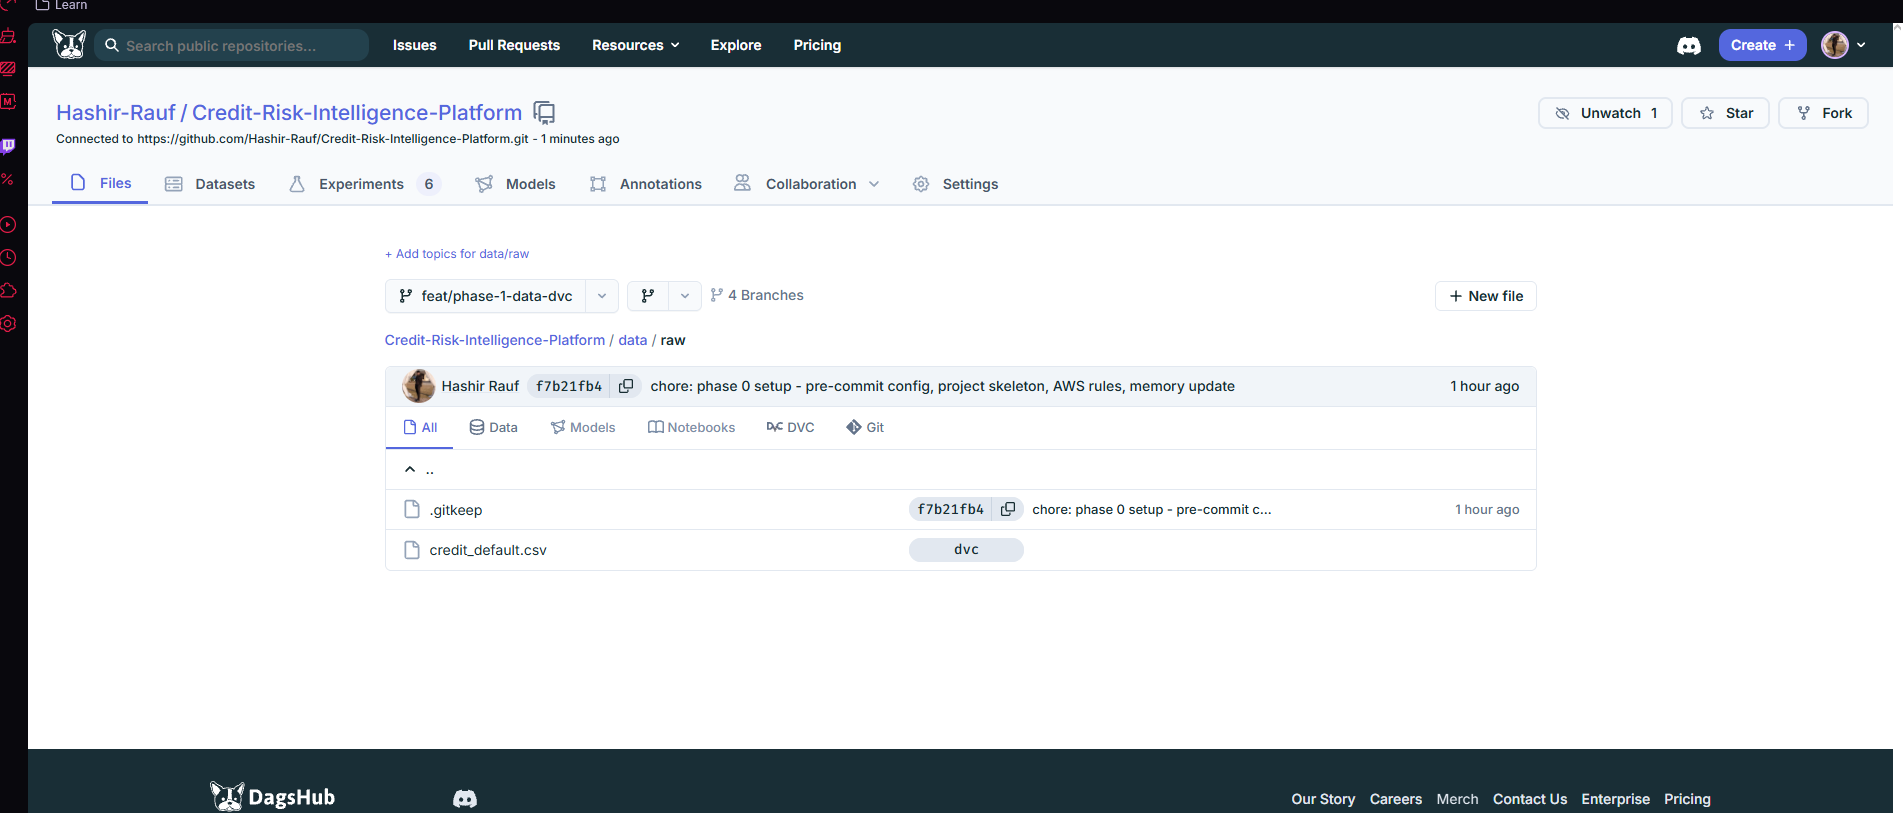
\includegraphics[width=0.9\linewidth]{phase-1/dagshub_data_view.png}
\caption{DagsHub mirror of the repository: the raw data file is listed as a DVC-tracked file (hash \texttt{a7e80c90...}).}
\end{figure}

% =====================================================================================================
\section{Modelling and results}
\label{sec:model}

\subsection{Features and model selection}
Preprocessing is a leakage-free \code{ColumnTransformer} fitted on the training split only. Besides the 20 raw inputs it engineers credit utilisation, payment-delay statistics (maximum, mean, number of delayed months) and bill/payment ratios, giving 32 model features. Three families were tuned with Optuna (20 trials each, three-fold cross-validation on the training split, seed 42) and compared on the \emph{validation} ROC-AUC.

\begin{table}[htbp]
\centering\small
\begin{tabular}{lrrrl}
\toprule
\hdr{Family} & \hdr{Val.\ ROC-AUC} & \hdr{CV ROC-AUC (mean $\pm$ std)} & \hdr{Trials} & \hdr{Selected}\\
\midrule
Logistic regression & 0.7634 & 0.7557 $\pm$ 0.0077 & 20 & \\
Random forest & 0.7922 & 0.7813 $\pm$ 0.0100 & 20 & \textbf{yes}\\
Histogram gradient boosting & 0.7925 & 0.7834 $\pm$ 0.0044 & 20 & \\
\bottomrule
\end{tabular}
\caption{Model families. The random forest is within 0.0003 validation ROC-AUC of gradient boosting and is the simpler model, so it was selected.}
\label{tab:families}
\end{table}

\textbf{Selected hyperparameters:} \code{n_estimators=200}, \code{max_depth=9}, \code{min_samples_leaf=2}, \code{max_features=sqrt}, \code{class_weight=balanced_subsample}.

\subsection{Evaluation metrics}
\begin{table}[htbp]
\centering\small
\begin{tabularx}{\linewidth}{lRR}
\toprule
\hdr{Metric (threshold 0.5)} & \hdr{Validation (n=4\,500)} & \hdr{Test (n=4\,500)}\\
\midrule
ROC-AUC & 0.7922 & \textbf{0.7883}\\
PR-AUC & 0.5739 & 0.5782\\
KS statistic & 0.4424 & 0.4401\\
Accuracy & 0.7769 & 0.7836\\
Precision & 0.4963 & 0.5094\\
Recall & 0.6070 & 0.6004\\
F1 & 0.5461 & 0.5512\\
Brier score & 0.1679 & 0.1667\\
Log loss & 0.5154 & 0.5125\\
\midrule
True positives / false positives & 604 / 613 & 598 / 576\\
True negatives / false negatives & 2\,892 / 391 & 2\,928 / 398\\
Positive rate & 0.2211 & 0.2213\\
\bottomrule
\end{tabularx}
\caption{Validation and held-out test metrics of the champion (registry version 1). The test split was read once, for this evaluation.}
\label{tab:metrics}
\end{table}

\textbf{Quality gate.} \code{reports/evaluation.json} records \code{gate.passed = true} (ROC-AUC 0.7883 against the 0.77 threshold). The same model, retrained from raw data on a different platform, reproduced every test metric exactly; only the validation log loss differed, by $1.1\times10^{-16}$.

\textbf{Calibration.} The Brier score and the calibration plot show the scores are not calibrated probabilities (mean score about 0.40 against 22\,\% real defaults). The API and UI therefore call the output a \emph{risk score}.

\begin{figure}[htbp]
\centering
\begin{subfigure}{0.48\linewidth}\includegraphics[width=\linewidth]{roc_curve_test.png}\caption{ROC curve}\end{subfigure}\hfill
\begin{subfigure}{0.48\linewidth}\includegraphics[width=\linewidth]{pr_curve_test.png}\caption{Precision-recall curve}\end{subfigure}\\[6pt]
\begin{subfigure}{0.48\linewidth}\includegraphics[width=\linewidth]{confusion_matrix_test.png}\caption{Confusion matrix}\end{subfigure}\hfill
\begin{subfigure}{0.48\linewidth}\includegraphics[width=\linewidth]{calibration_test.png}\caption{Calibration}\end{subfigure}
\caption{Test-split evaluation plots of the champion.}
\end{figure}

\subsection{Explainability}
Explanations use a model-agnostic SHAP permutation explainer; contributions are in log-odds and add up exactly to the score. Table~\ref{tab:shap} lists the global ranking. Repayment behaviour dominates: the worst payment delay, the number of delayed months and the latest repayment status are the top three drivers. Sensitive attributes never appear because they are not inputs. Explanations describe the model's behaviour, not causes in the real world.

\begin{table}[htbp]
\centering\small
\begin{tabularx}{0.85\linewidth}{rXr}
\toprule
\hdr{Rank} & \hdr{Feature} & \hdr{Mean $|$contribution$|$}\\
\midrule
1 & Worst payment delay (months) & 0.1564\\
2 & Months with a delayed payment & 0.1268\\
3 & Repayment status, month 1 & 0.1088\\
4 & Average payment delay (months) & 0.0993\\
5 & Payment amount, month 1 & 0.0678\\
6 & Credit limit & 0.0638\\
7 & Bill amount, month 1 & 0.0534\\
8 & Credit utilisation, 6-month average & 0.0497\\
9 & Payment amount, month 4 & 0.0470\\
10 & Credit utilisation, latest month & 0.0453\\
\bottomrule
\end{tabularx}
\caption{Global SHAP importance (100 sampled test rows, 50 background rows).}
\label{tab:shap}
\end{table}

\begin{figure}[htbp]
\centering
\includegraphics[width=0.85\linewidth]{explanations.png}
\caption{Explanation summary produced by the pipeline.}
\end{figure}

\subsection{Fairness audit}
\label{sec:fairness}
Group metrics were computed on the test split for sex, marital status and age band (the 60+ band has only 44 customers and is excluded from gaps). The ablation retrains the model \emph{with} the sensitive attributes: test ROC-AUC becomes 0.7880 against 0.7883 without them, a change of $-0.0003$, far below the 0.005 materiality threshold, so excluding them costs nothing measurable.

\begin{table}[htbp]
\centering\small
\begin{tabularx}{\linewidth}{llrrrrrr}
\toprule
\hdr{Attribute} & \hdr{Group} & \hdr{n} & \hdr{Approval} & \hdr{TPR} & \hdr{FPR} & \hdr{AUC} & \hdr{Default rate}\\
\midrule
Age band & $<$30 & 1\,390 & 0.699 & 0.666 & 0.194 & 0.805 & 0.226\\
 & 30--39 & 1\,760 & 0.773 & 0.589 & 0.139 & 0.802 & 0.195\\
 & 40--49 & 950 & 0.746 & 0.558 & 0.159 & 0.767 & 0.238\\
 & 50--59 & 356 & 0.697 & 0.538 & 0.204 & 0.722 & 0.298\\
\midrule
Marital status & married & 2\,053 & 0.741 & 0.581 & 0.157 & 0.788 & 0.241\\
 & single & 2\,392 & 0.738 & 0.620 & 0.170 & 0.790 & 0.204\\
 & other & 50 & 0.700 & 0.615 & 0.189 & 0.850 & 0.260\\
\midrule
Sex & male & 1\,839 & 0.711 & 0.610 & 0.190 & 0.778 & 0.234\\
 & female & 2\,661 & 0.758 & 0.593 & 0.147 & 0.795 & 0.212\\
\bottomrule
\end{tabularx}
\caption{Group metrics of the champion (no sensitive inputs). ``Approval'' is the share not flagged at the threshold.}
\end{table}

\begin{table}[htbp]
\centering\small
\begin{tabularx}{\linewidth}{lXrrrrr}
\toprule
\hdr{Attribute} & \hdr{Model} & \hdr{Approval gap} & \hdr{TPR gap} & \hdr{FPR gap} & \hdr{AUC gap} & \hdr{Disp.\ impact}\\
\midrule
\multirow{2}{*}{Age band} & without sensitive inputs & 0.0767 & 0.1279 & 0.0650 & 0.0830 & 0.901\\
 & with sensitive inputs & 0.0739 & 0.1025 & 0.0577 & 0.0834 & 0.904\\
\multirow{2}{*}{Marital status} & without & 0.0414 & 0.0387 & 0.0327 & 0.0624 & 0.944\\
 & with & 0.0458 & 0.0324 & 0.0320 & 0.0606 & 0.939\\
\multirow{2}{*}{Sex} & without & 0.0471 & 0.0173 & 0.0434 & 0.0166 & 0.938\\
 & with & 0.0513 & 0.0290 & 0.0453 & 0.0159 & 0.933\\
\bottomrule
\end{tabularx}
\caption{Disparities between the best and worst group. Report-only failures: age-band TPR gap, age-band AUC gap and marital-status AUC gap. Excluding the attributes does not remove the gaps, because other features act as proxies; the gaps are monitored and a challenger may not widen them by more than 0.02.}
\end{table}

% =====================================================================================================
\section{Testing, CI and orchestration}
\label{sec:pipelines}

\subsection{Continuous integration}
\code{ci.yml} runs on every push and pull request: lint (ruff, black), tests with coverage, bandit, pip-audit, gitleaks on the full history, and a Docker build with a Trivy scan of the API, monitor and frontend images; the frontend job runs 14 unit and 7 browser tests. The suite has about 500 tests, including 67 for the API (valid, malformed, missing and wrongly typed input), data, model, integration and regression tests (a candidate may not drop more than a set margin against stored baseline metrics). The required check \texttt{CI passed} blocks merging.

\begin{table}[htbp]
\centering\small
\begin{tabularx}{\linewidth}{L{3.0cm}L{3.6cm}L{2.4cm}X}
\toprule
\hdr{Run} & \hdr{Branch / commit} & \hdr{Result} & \hdr{Notes}\\
\midrule
45229774869 & \texttt{feat/phase-3-ci} & green & first run: tests 7.3\,min, lint 0.2\,min\\
45231592266 & \texttt{evidence/ci-red-demo} & \textbf{red (intended)} & one deliberately failing test; the required check failed, so the merge button stays blocked\\
45233201820 & same branch, fix commit & green & failing test removed\\
45317211962 & \texttt{feat/phase-4-serving} & green & lint 12\,s, tests 7\,min 31\,s, Docker 2\,min 9\,s, frontend 57\,s\\
\bottomrule
\end{tabularx}
\caption{CI evidence: a red and a green run with the same gate.}
\end{table}

A commit containing a fake token and a fake private key was refused by two independent pre-commit hooks (\code{detect-private-key} and gitleaks); \code{HEAD} did not move.

\subsection{Pipeline orchestration (Airflow and Kubeflow)}
One Airflow trigger runs \code{ml_orchestrator_dag}: fetch data $\rightarrow$ validate (failure stops the DAG) $\rightarrow$ DVC push $\rightarrow$ trigger Kubeflow run $\rightarrow$ poll $\rightarrow$ check gate $\rightarrow$ notify, with retries, retry delay and logging. Airflow owns schedule, data and trigger; Kubeflow owns the containerised ML graph; they never run duplicate work. Deterministic failures use an exit-code contract (2 = validation failed, 3 = gate rejected) and are not retried.

\begin{table}[htbp]
\centering\small
\begin{tabularx}{\linewidth}{L{3.1cm}L{2.6cm}X}
\toprule
\hdr{Scenario} & \hdr{Parameters} & \hdr{Outcome}\\
\midrule
Real data & source = uci & 7/7 tasks succeeded, one Kubeflow run, gate passed, model registered as \code{staging} v4; \code{champion} untouched\\
Corrupt data & source = corrupt & \code{validate} failed on attempt 1 (exit 2, no retry); every downstream task \code{upstream_failed}; nothing reached DVC or Kubeflow\\
Strict gate & strict\_gate = true & Kubeflow run succeeded but \code{package_register} was skipped; \code{check_gate} failed once (exit 3, no retry); zero versions registered\\
Transient failure & retry\_demo = true & first attempt raised the deliberate error and was retried; the second succeeded; the Kubeflow run started exactly once\\
\bottomrule
\end{tabularx}
\caption{Phase 5 acceptance runs, executed against the shared DagsHub MLflow and DVC remote.}
\end{table}

\begin{figure}[htbp]
\centering
\begin{subfigure}{0.48\linewidth}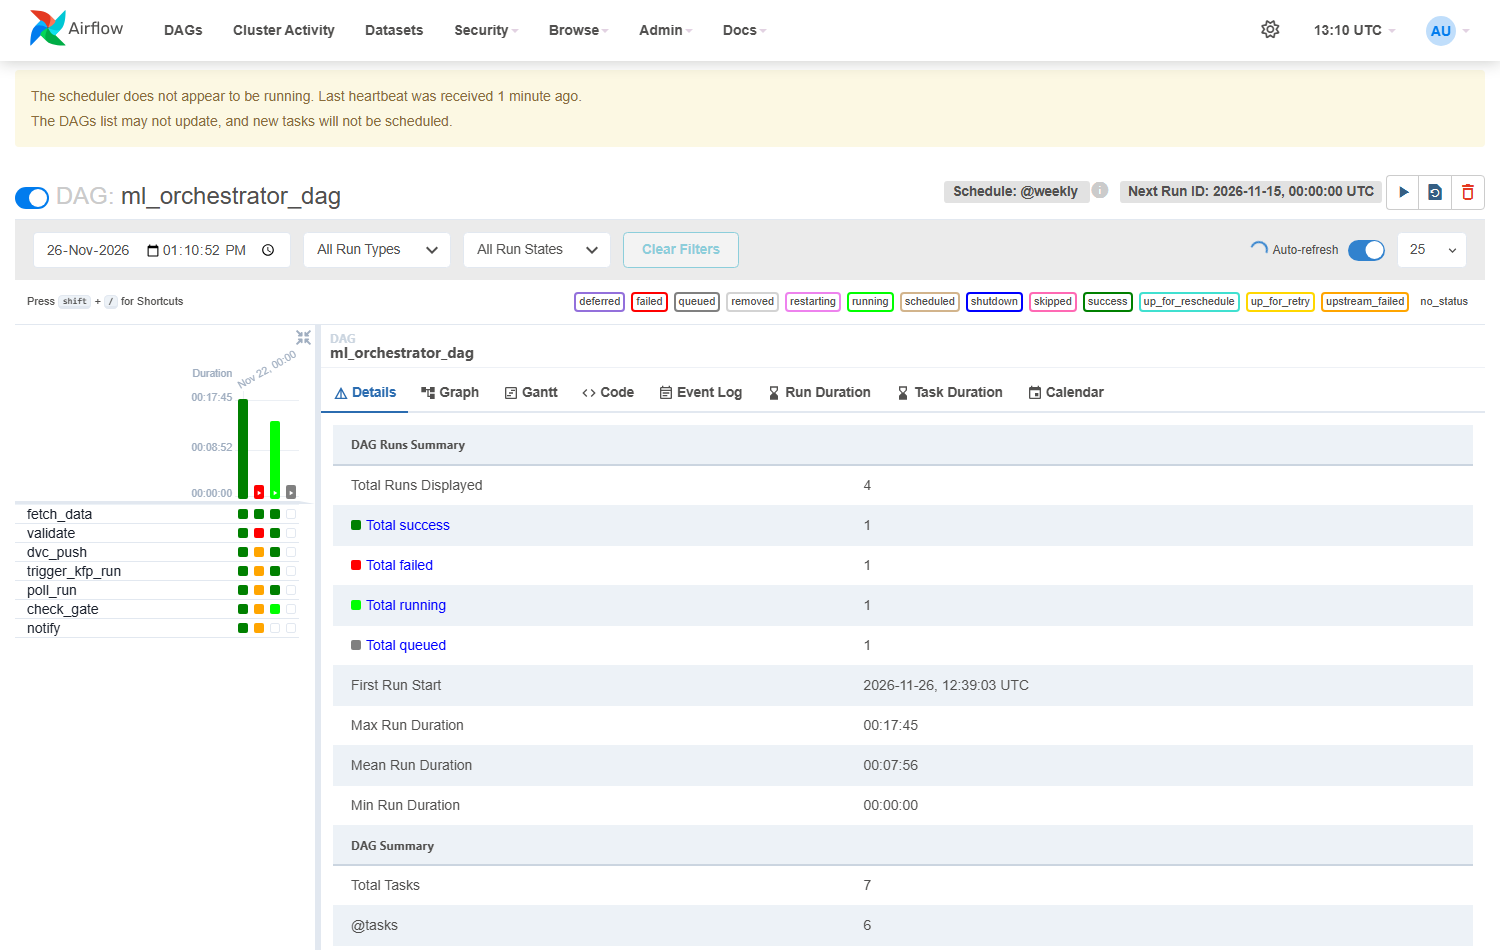
\includegraphics[width=\linewidth]{phase-5/screenshots/airflow-01-grid.png}\caption{Airflow grid of runs}\end{subfigure}\hfill
\begin{subfigure}{0.48\linewidth}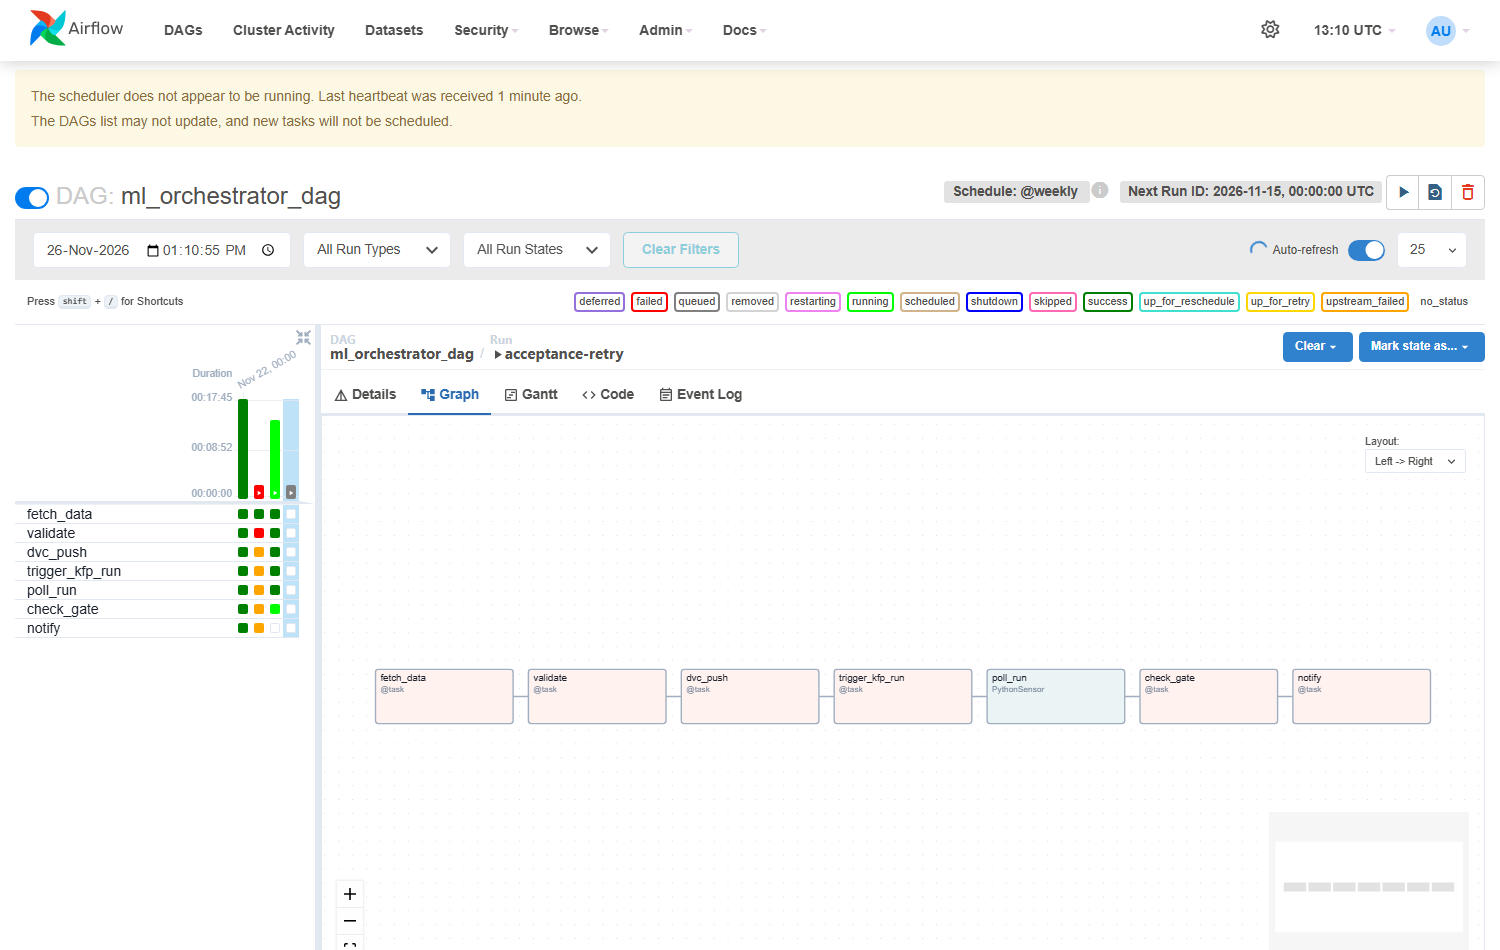
\includegraphics[width=\linewidth]{phase-5/screenshots/airflow-02-real-uci-graph.png}\caption{Real-data run, all tasks green}\end{subfigure}\\[6pt]
\begin{subfigure}{0.48\linewidth}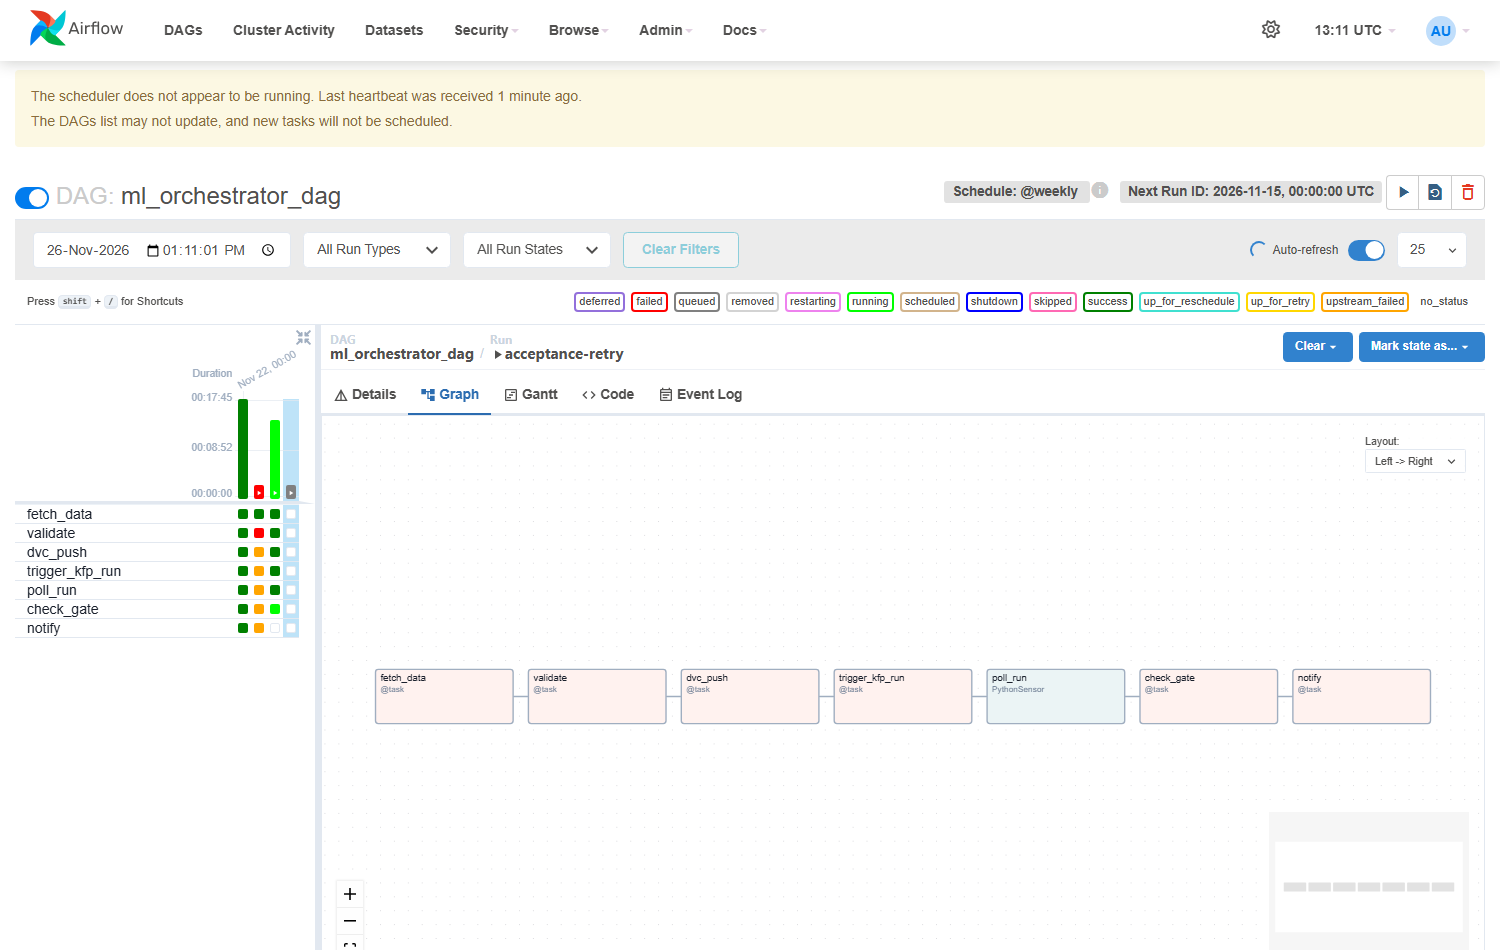
\includegraphics[width=\linewidth]{phase-5/screenshots/airflow-03-corrupt-graph.png}\caption{Corrupt data stops at validation}\end{subfigure}\hfill
\begin{subfigure}{0.48\linewidth}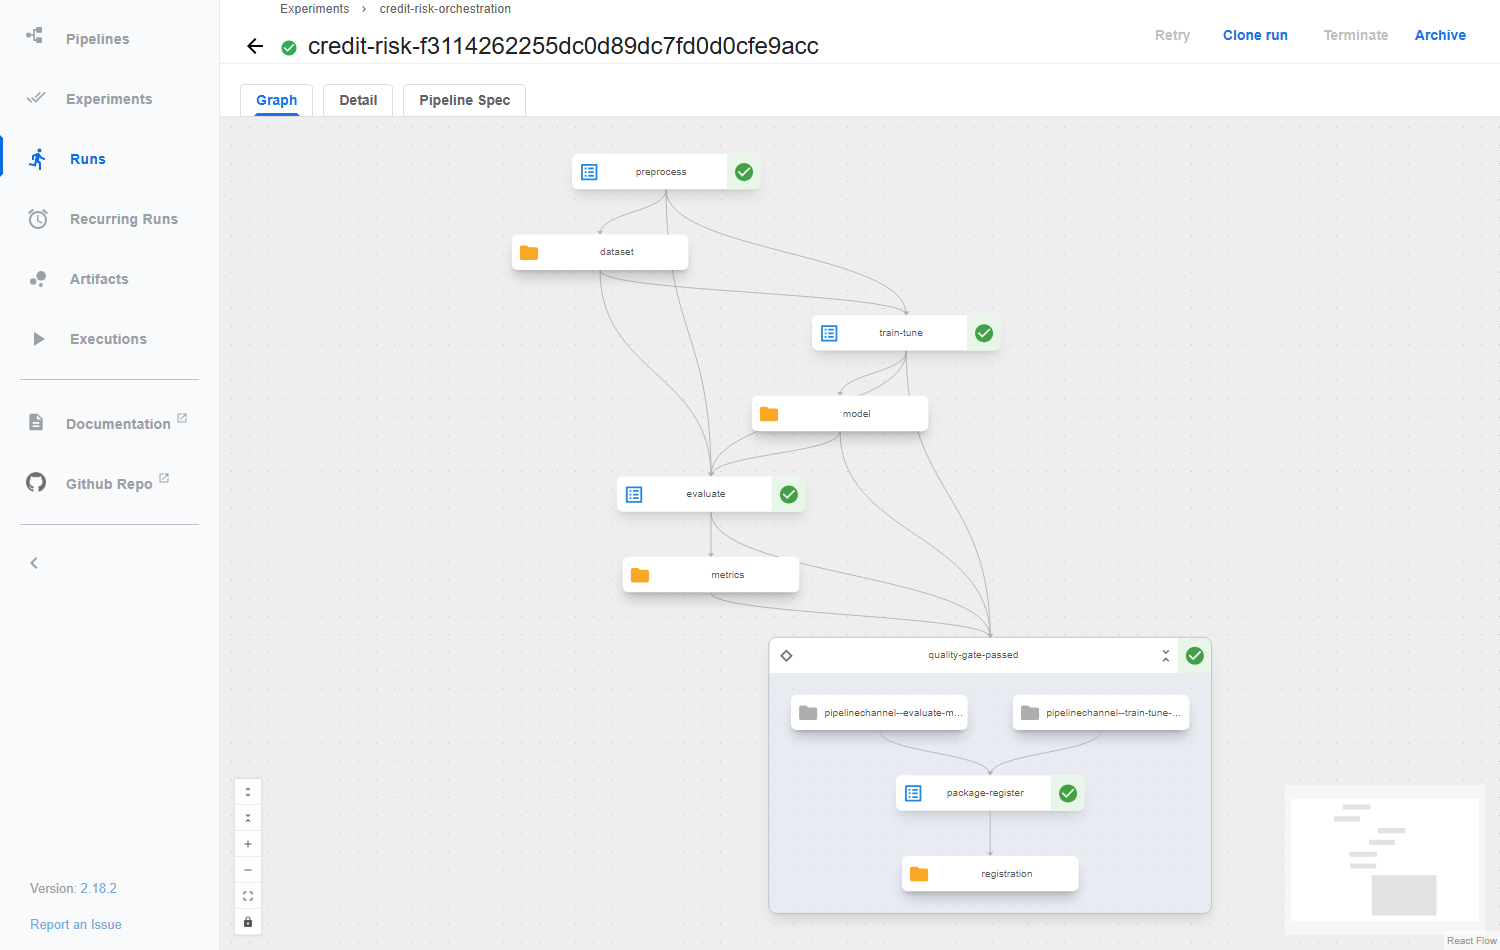
\includegraphics[width=\linewidth]{phase-5/screenshots/kfp-02-real-uci-run-graph.png}\caption{Kubeflow run graph}\end{subfigure}
\caption{Orchestration evidence.}
\end{figure}

\begin{figure}[htbp]
\centering
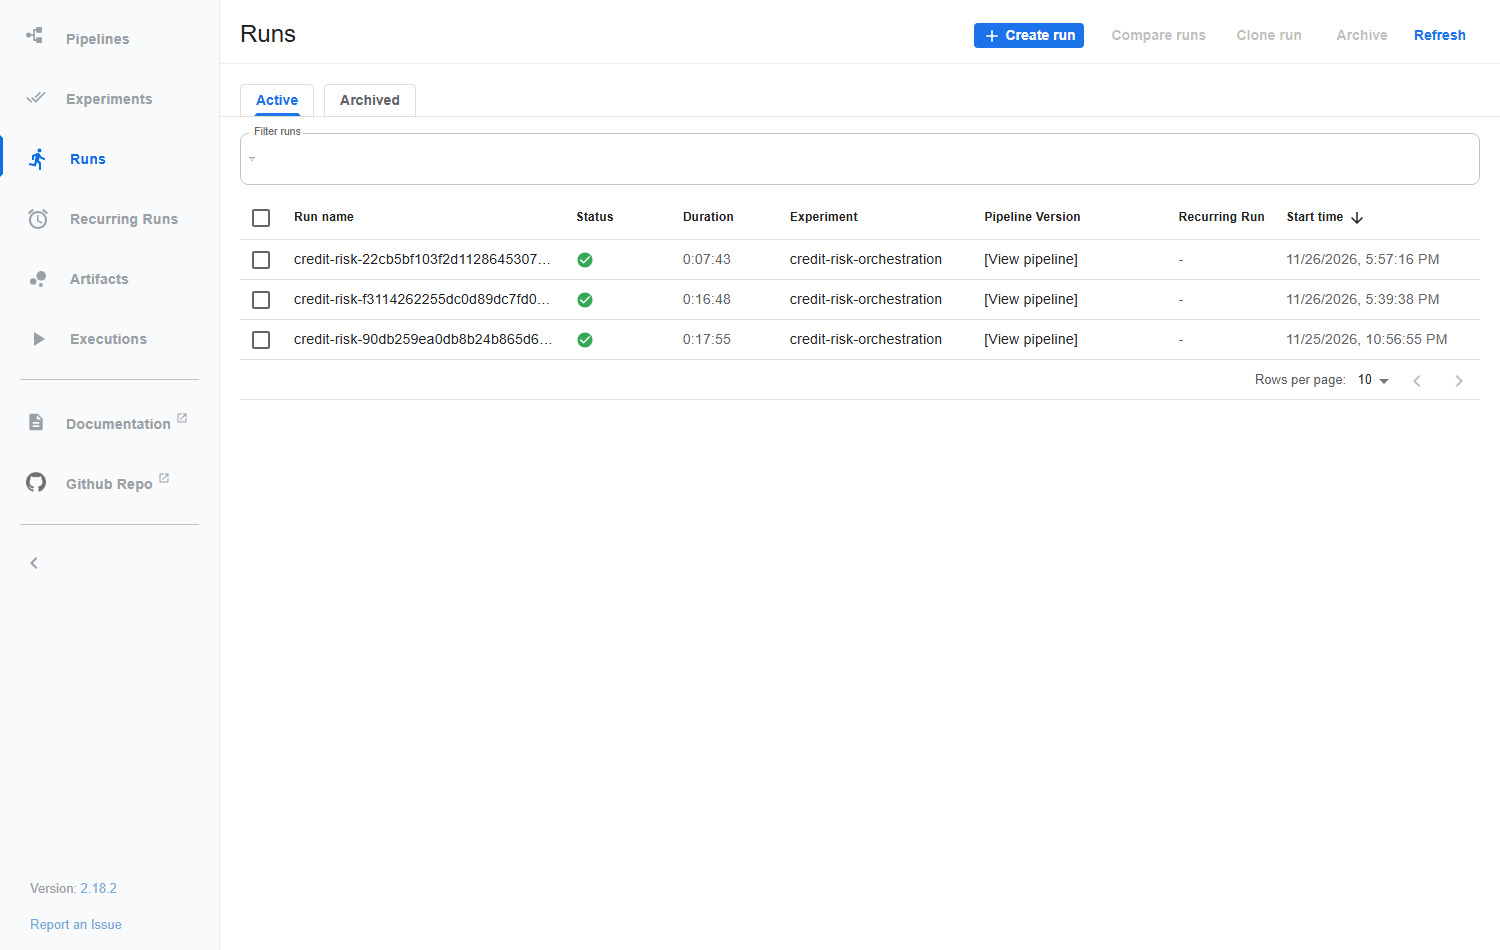
\includegraphics[width=0.9\linewidth]{phase-5/screenshots/kfp-01-runs.png}
\caption{Kubeflow Pipelines run list.}
\end{figure}

The first live run found bugs that no test had: a request-id collision with a teammate's run on the shared server, retries of non-retryable failures, and helper errors that were invisible in the task log. All were fixed and documented under \code{docs/evidence/phase-5/found-and-fixed/}.

% =====================================================================================================
\section{Serving and web interface}
\label{sec:serving}

The Flask API exposes \code{/health}, \code{/model-info}, \code{/predict}, \code{/explain} and \code{/metrics}. Inputs are validated against the model's feature schema (errors name the field): malformed JSON returns 400, a wrong content type 415, an oversize body 413, invalid fields 422 and a missing or wrong API key 401. The container runs as a non-root user (uid 10001). The score returned is a \emph{risk score}; each response carries a disclaimer.

\subsection{Example request and response (live AWS service)}
The request body contains only the 20 model inputs, with no name, e-mail or sensitive attribute. \texttt{<public-ip>} is the task address printed by \code{infra/aws/endpoint.sh}.

\begin{lstlisting}
$ curl -s http://<public-ip>:8000/health
{"status":"ok","model_loaded":true,"model_version":"1","uptime_s":338.6}

$ curl -s -o /dev/null -w "%{http_code}\n" -X POST http://<public-ip>:8000/predict \
       -H "Content-Type: application/json" -d @scripts/sample_predict.json
401                                   # no X-API-Key header: refused

$ curl -s -X POST http://<public-ip>:8000/predict -H "X-API-Key: $API_KEY" \
       -H "Content-Type: application/json" -d @scripts/sample_predict.json
{"request_id":"9b8a832f63d7408f9ea1b87f00abfcc9","model_version":"1","threshold":0.5,
 "score_type":"uncalibrated_risk_score",
 "predictions":[{"risk_score":0.612094,"prediction":1}],"ignored_fields":[],
 "disclaimer":"Educational model for a university course. Not a real lending
  decision tool. risk_score is a model ranking score, not a calibrated probability
  of default."}
\end{lstlisting}

The request file used above is:
\begin{lstlisting}
{"LIMIT_BAL": 50000, "EDUCATION": 3, "PAY_1": 1, "PAY_2": 2, "PAY_3": 0, "PAY_4": 0,
 "PAY_5": 0, "PAY_6": 0, "BILL_AMT1": 49000, "BILL_AMT2": 48000, "BILL_AMT3": 47000,
 "BILL_AMT4": 46000, "BILL_AMT5": 45000, "BILL_AMT6": 44000, "PAY_AMT1": 1500,
 "PAY_AMT2": 1000, "PAY_AMT3": 1000, "PAY_AMT4": 1200, "PAY_AMT5": 1000, "PAY_AMT6": 1000}
\end{lstlisting}

\subsection{Web interface}
The Next.js interface has a blue sidebar, stat cards and a scoring form built from the API's schema. Its server side calls the API and attaches the key, so the browser never sees it; a Playwright test proves that no request, header, body, HTML or script contains the key while the server still sends it. The screenshots below were taken from the interface running on AWS.

\begin{figure}[htbp]
\centering
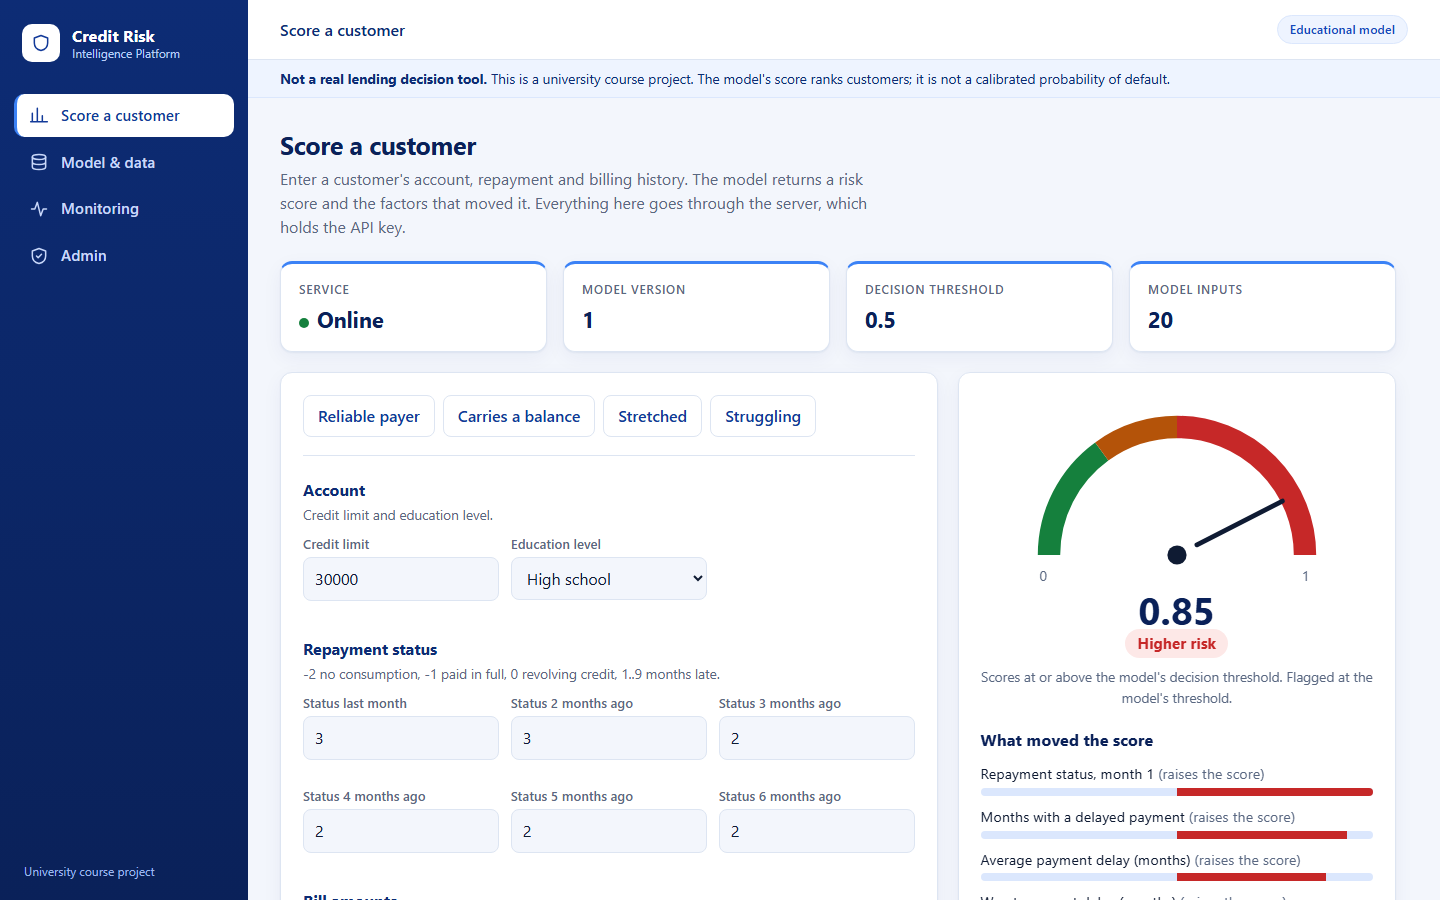
\includegraphics[width=\linewidth]{phase-6/screenshots/aws-02-score-higher-risk.png}
\caption{Scoring page (live AWS): the ``Struggling'' example customer scores 0.85, band \emph{Higher risk}, with the factors that moved the score. The stat cards show service status, model version, threshold and number of inputs.}
\end{figure}

\begin{figure}[htbp]
\centering
\begin{subfigure}{0.48\linewidth}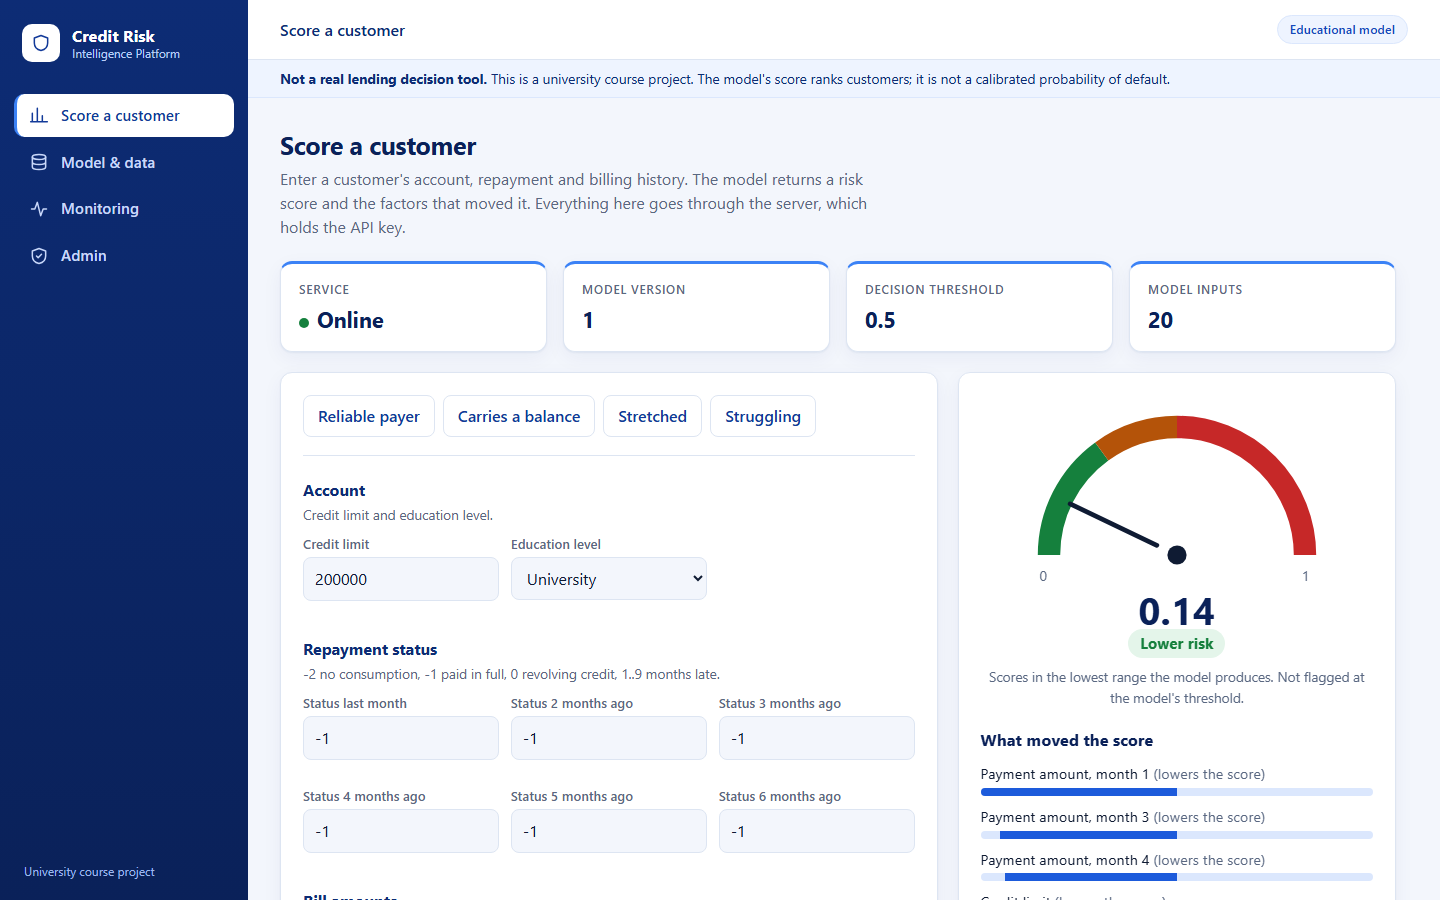
\includegraphics[width=\linewidth]{phase-6/screenshots/aws-03-score-lower-risk.png}\caption{``Reliable payer'': \emph{Lower risk}}\end{subfigure}\hfill
\begin{subfigure}{0.48\linewidth}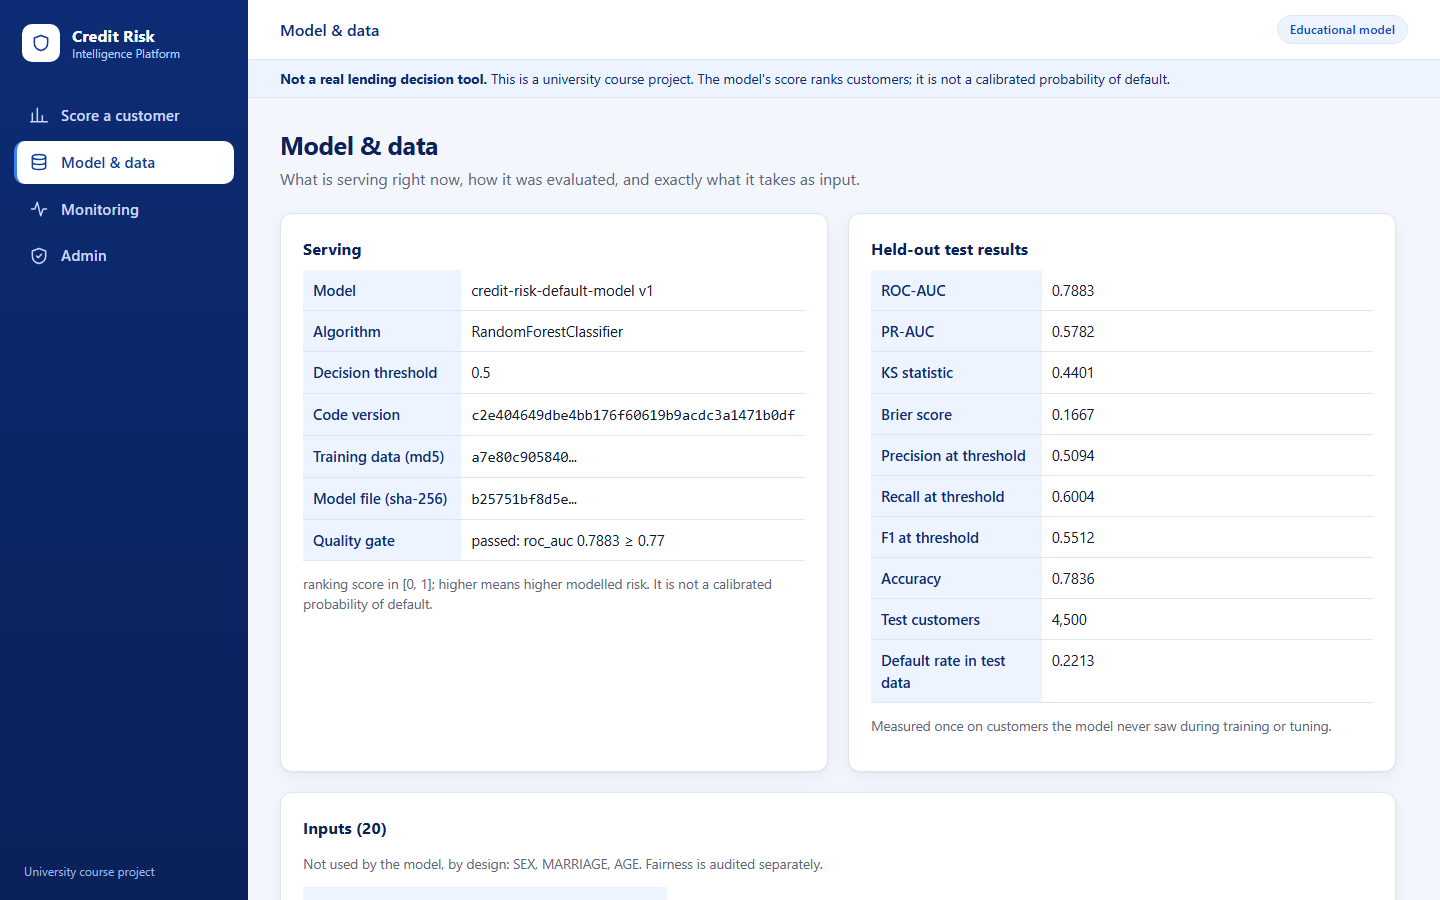
\includegraphics[width=\linewidth]{phase-6/screenshots/aws-04-model-and-data.png}\caption{Model \& data: serving version, git SHA, test metrics, quality gate}\end{subfigure}\\[6pt]
\begin{subfigure}{0.48\linewidth}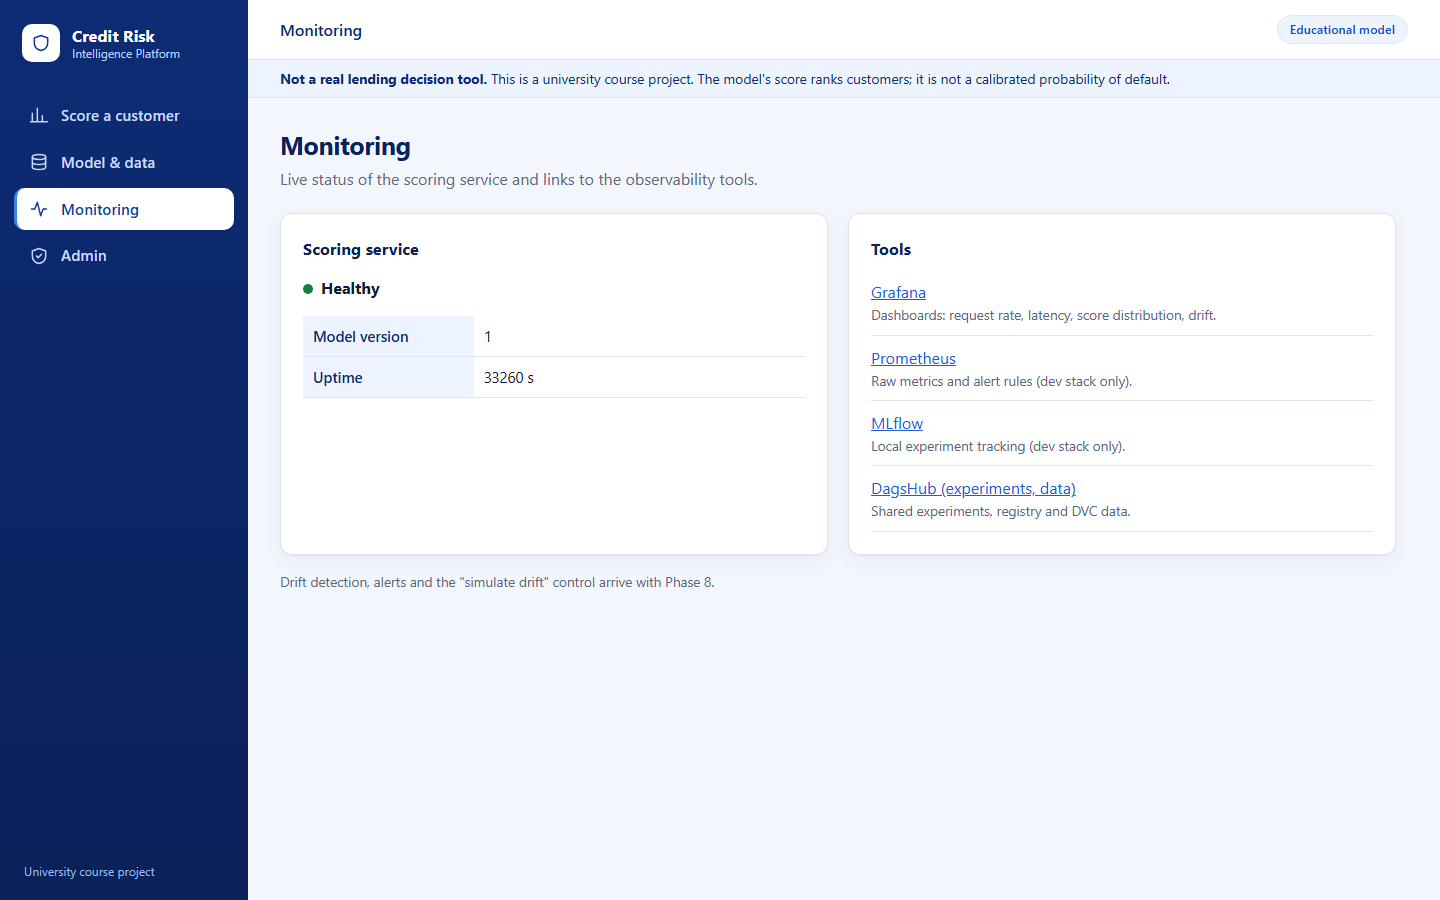
\includegraphics[width=\linewidth]{phase-6/screenshots/aws-05-monitoring.png}\caption{Monitoring: live service health}\end{subfigure}\hfill
\begin{subfigure}{0.48\linewidth}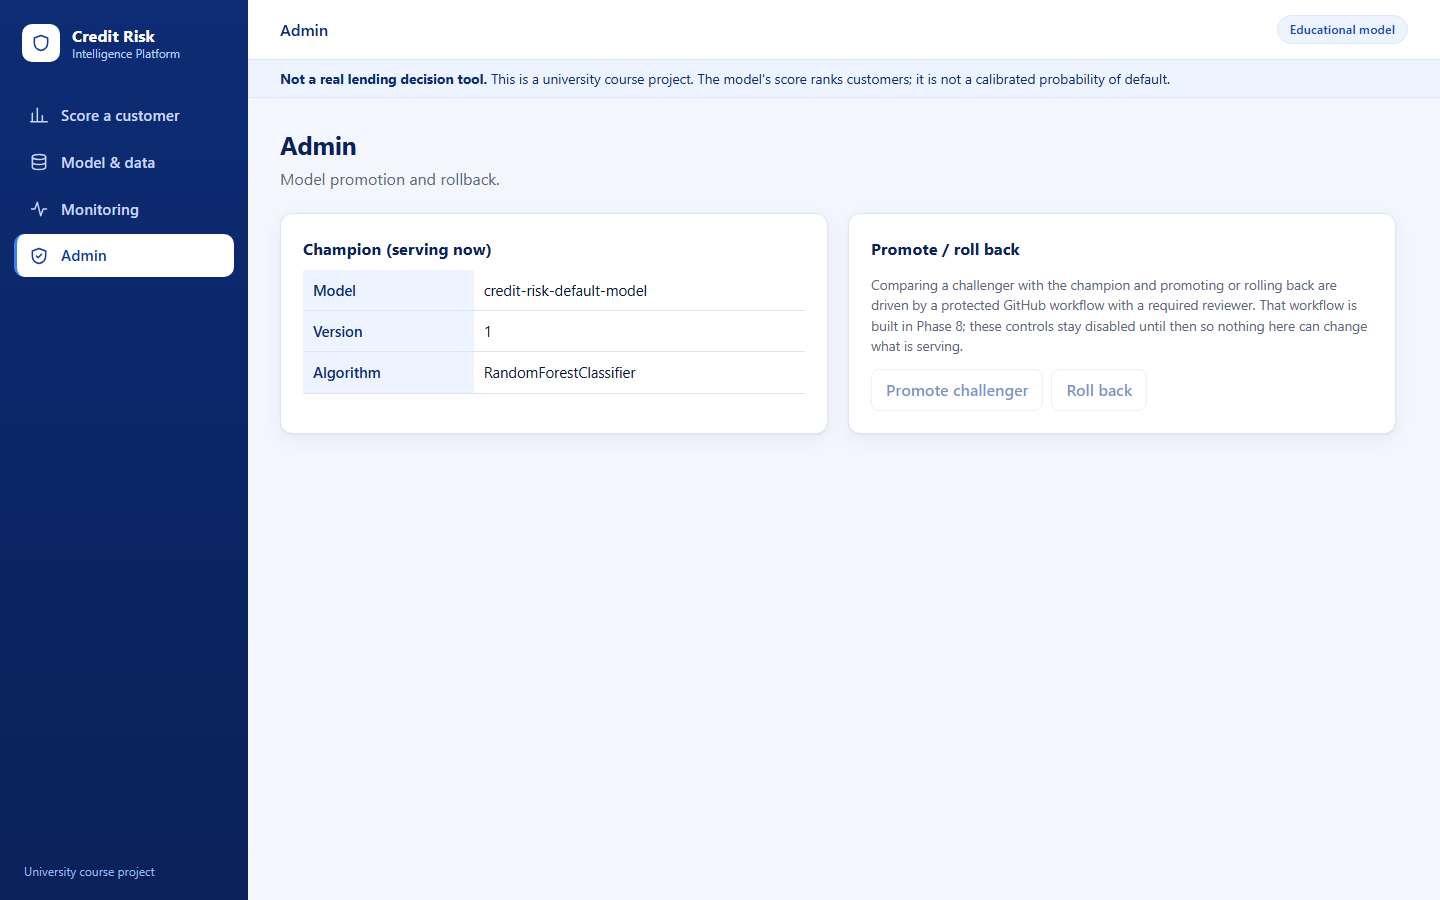
\includegraphics[width=\linewidth]{phase-6/screenshots/aws-06-admin.png}\caption{Admin: champion information}\end{subfigure}
\caption{More screens of the deployed interface.}
\end{figure}

\begin{figure}[htbp]
\centering
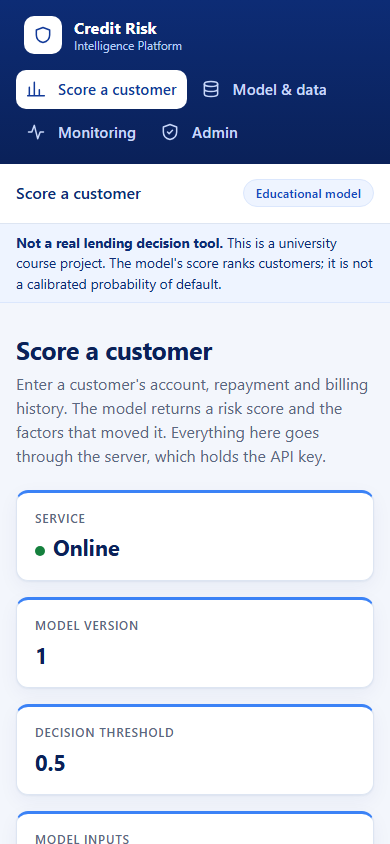
\includegraphics[width=0.3\linewidth]{phase-6/screenshots/aws-07-phone-width.png}
\caption{The layout at phone width (390\,px): the sidebar becomes a top bar.}
\end{figure}

% =====================================================================================================
\section{AWS deployment and continuous delivery}
\label{sec:aws}

\subsection{What runs on AWS}
The Region is \code{ap-southeast-2} and the account is on the Free plan, so only credits are used. Two CloudFormation stacks create everything; \code{teardown.sh} deletes both and then lists what is left.

\begin{table}[htbp]
\centering\small
\begin{tabularx}{\linewidth}{L{3.6cm}X}
\toprule
\hdr{Service} & \hdr{Use}\\
\midrule
ECS Fargate & one task (0.5\,vCPU / 1\,GB) with two containers: the API and the web UI (non-essential, so a UI crash never stops the API); circuit breaker with automatic rollback\\
ECR & two repositories, immutable tags (git SHA), scan on push\\
Secrets Manager & generated API key and prediction-log salt, never typed or stored in git\\
S3 & artifact bucket (encrypted, TLS-only, lifecycle rules for logs and reports)\\
CloudWatch & log group, metric filters and two alarms (5xx rate, p95 latency) notifying through SNS\\
IAM & execution role, task role (read models, write prediction logs), GitHub OIDC deploy role scoped to one repository and one environment\\
Security group & the API port is open to one operator address only; the UI port was deliberately opened publicly for the demonstration\\
\bottomrule
\end{tabularx}
\caption{AWS services. There is no load balancer and no NAT gateway; the public IP changes on every deployment.}
\end{table}

\subsection{Delivery pipeline}
\begin{enumerate}
\item CI succeeds on \code{main}; the Deploy workflow starts and waits for a required reviewer to approve the \code{production} environment (the human gate).
\item The job assumes the deploy role through GitHub OIDC (no stored AWS keys), pulls the model from DVC, and refuses to continue unless the quality gate in \code{reports/evaluation.json} passed.
\item It builds the API image (model baked in) and the UI image, scans both with Trivy (HIGH and CRITICAL with a fix fail the run), and pushes them to ECR tagged with the git SHA.
\item \code{scripts/aws_ecs_deploy.sh} registers a new task-definition revision, updates the service, waits for stability, and runs the smoke test (health, a 401 without the key, an authenticated prediction, the UI check). On failure it points the service back at the previous revision.
\item Only after success is the \code{champion} alias moved when a model version was supplied.
\end{enumerate}

\subsection{Evidence}
The CD workflow ran from \code{main} after the pull-request merge: every step succeeded (OIDC login, DVC pull, gate check, API and UI image builds, Trivy, ECR push, deploy and smoke test; first full run 5\,min 23\,s). The service then reported \code{ACTIVE}, desired 1, running 1, rollout \code{COMPLETED}, with both containers \code{RUNNING}. From outside: \code{GET /} returned 200 with the scoring form, \code{GET /api/health} returned \verb|{"frontend":"ok","api":"ok","api_status":200}|, and a prediction through the UI worked without any key in the browser. The 401, 200 and prediction responses are listed in Section~\ref{sec:serving}.

Verified state of the running service (read with the AWS API after the deployment):
\begin{lstlisting}
service credit-risk-api   status ACTIVE   desired 1   running 1   rollout COMPLETED
task definition credit-risk-api:5   cpu 512   memory 1024
containers   api: RUNNING   frontend: RUNNING
images       credit-risk-api:<git-sha>   credit-risk-frontend:<git-sha>   (same commit)
alarms       credit-risk-api-5xx: OK   credit-risk-api-p95-latency: OK
\end{lstlisting}

\subsection{Rollback run}
The Rollback workflow was run with target \code{previous}. It moved the service from task-definition revision 6 to revision 5, waited for the service to be stable and ran the same smoke test as a deployment: \code{/health} answered, a prediction without the key was rejected, a prediction with the key succeeded and the web UI answered.
\begin{figure}[htbp]
\centering
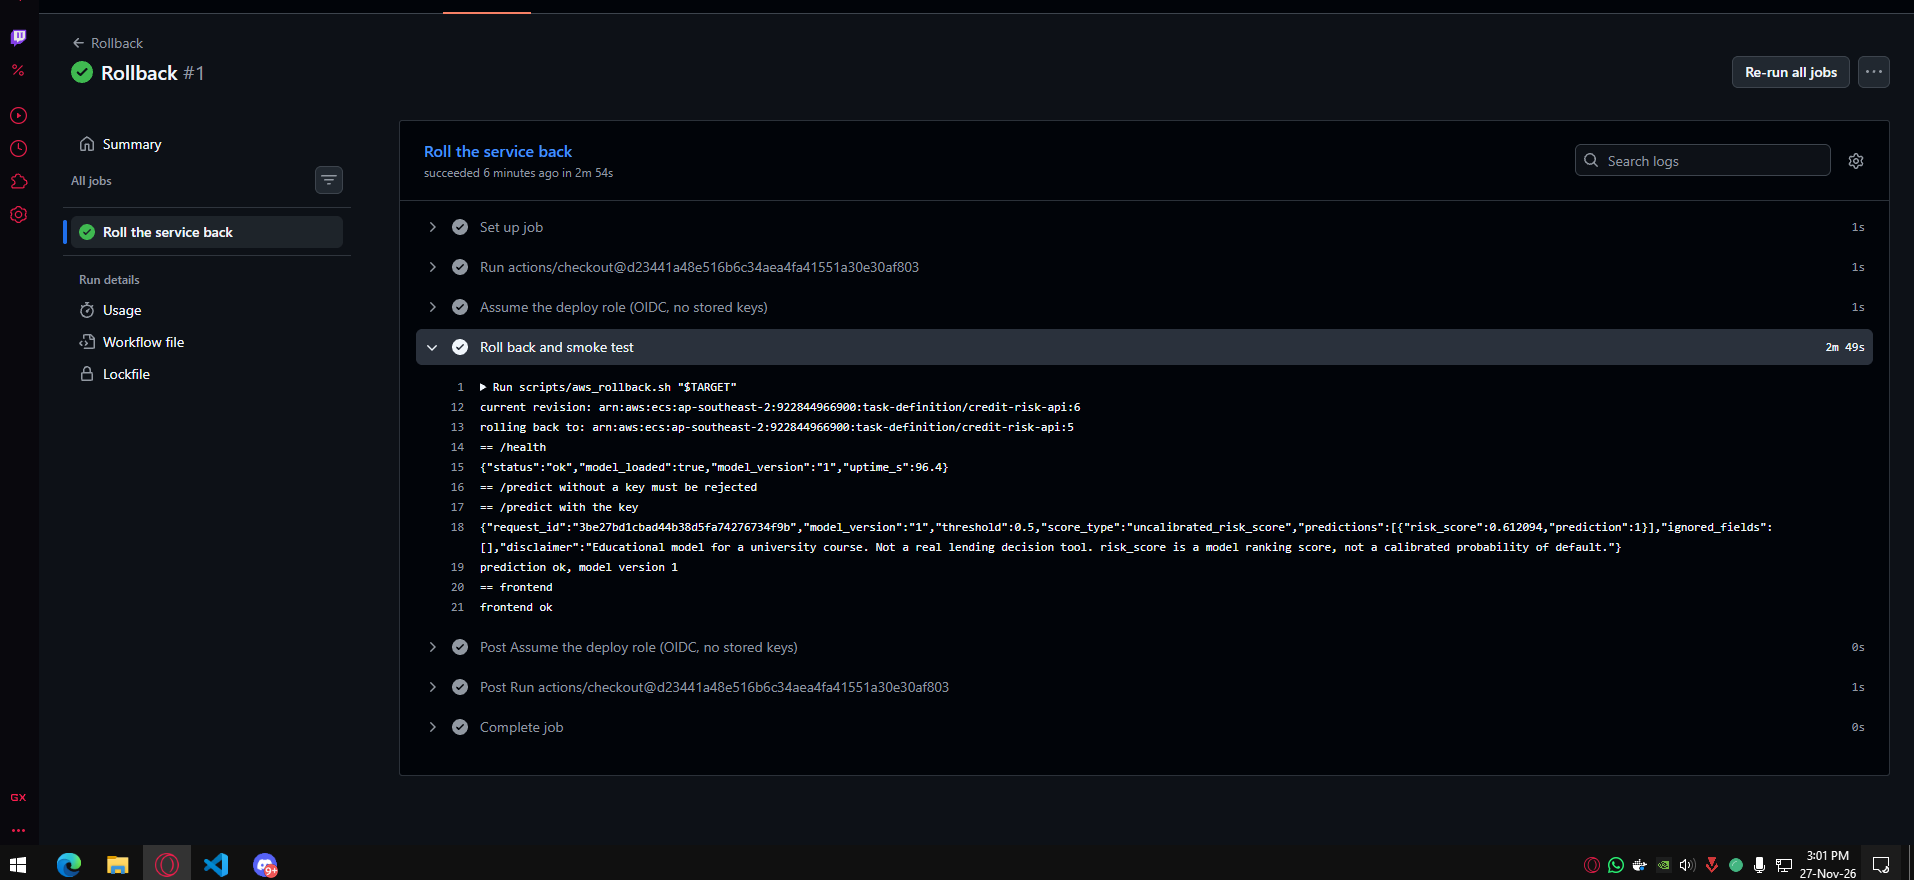
\includegraphics[width=\linewidth]{phase-6/screenshots/rollback-run.png}
\caption{Rollback \#1 (GitHub Actions): current revision 6, rolling back to revision 5, then the smoke test passes.}
\end{figure}

\subsection{Alarm}
The 5xx alarm was put into the ALARM state with a manual state change (\code{aws cloudwatch set-alarm-state}), because the service does not produce HTTP 5xx on purpose; the metric filter and threshold were therefore not exercised by traffic. The alarm history shows the transition and the automatic return to OK at the next evaluation: \code{OK -> ALARM} at 14:59:30 and \code{ALARM -> OK} at 15:00:02 (UTC+5, 27 November). The e-mail notification was not received because the SNS subscription was still pending confirmation.
\begin{figure}[htbp]
\centering
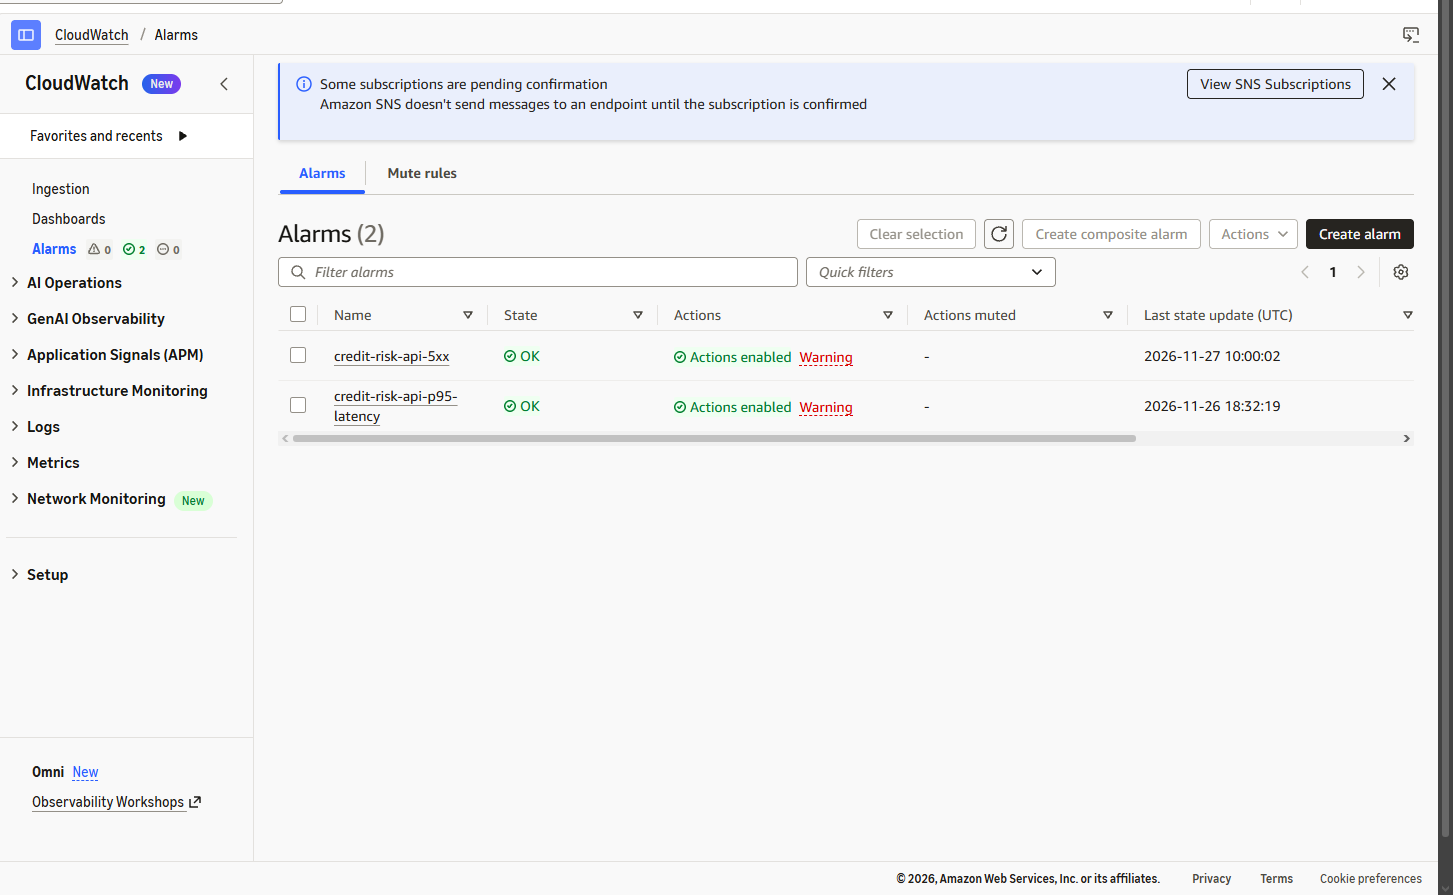
\includegraphics[width=\linewidth]{phase-6/screenshots/cloudwatch-alarms.png}
\caption{CloudWatch alarms after the test: both alarms are OK; the 5xx alarm's last state update (10:00:02 UTC) is its return from the manual ALARM.}
\end{figure}

\subsection{Problems the live deployment found (all fixed)}
\begin{longtable}{L{5.4cm}L{8.6cm}}
\toprule
\hdr{Problem} & \hdr{Cause and fix}\\
\midrule\endhead
OIDC login refused (\code{AccessDenied}) & GitHub now puts numeric owner and repository IDs into the token subject; the trust policy expected the plain form. Found by reading the subject in CloudTrail; the role now accepts both forms (exact repository and environment only)\\
DVC pull failed & the S3 remote lacked two model objects present only in the local cache; pushed\\
Push step failed (\code{ecr:ListImages} denied) & the step verified the push with a permission the deploy role intentionally lacks; it now uses \code{DescribeImages}\\
\code{Permission denied} on the deploy script & scripts created on Windows were not executable in git; mode fixed\\
Smoke test failed on a machine without Python & the check used \code{python3}; now \code{jq}; the script also stopped printing the key outside GitHub Actions\\
Page unreachable after an ISP change & the security group allowed only the operator's old IP; updated through the stack\\
\bottomrule
\end{longtable}

\subsection{Cost}
The smallest sizes are used: about \$0.60 per day while the task runs (0.5\,vCPU, 1\,GB and a public IPv4 address), taken from the credits on the Free plan; an AWS budget exists in the Billing console. Cost Explorer (20--26 November, daily, grouped by service) shows a total of -\$0.00: the charges so far are offset by the credits, and billing data lags by up to a day (Figure~\ref{fig:cost}). The resources are removed after the demonstration (Section~\ref{sec:cleanup}).

\begin{figure}[htbp]
\centering
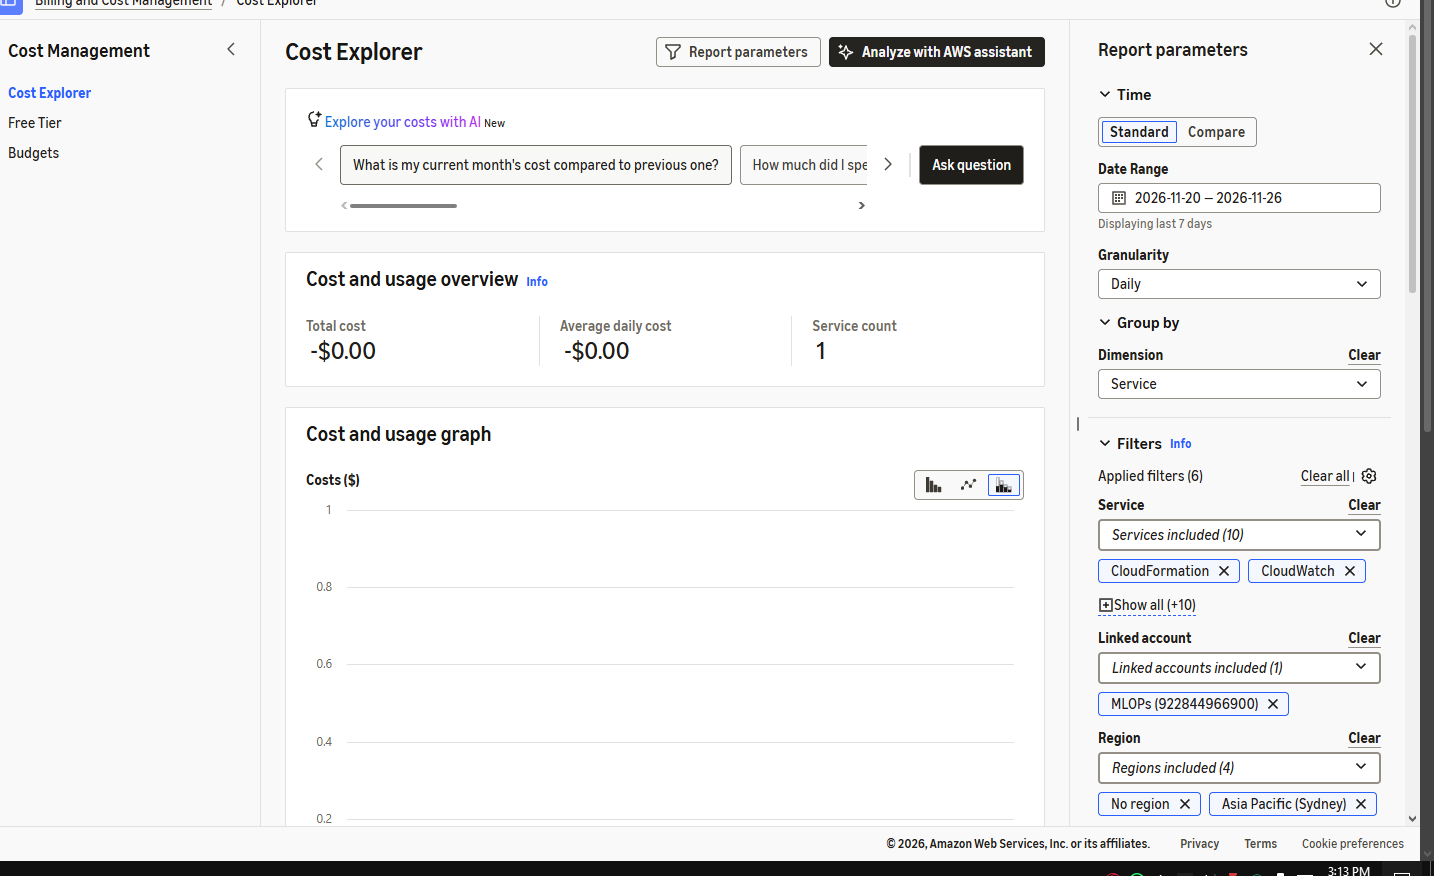
\includegraphics[width=0.85\linewidth]{phase-6/screenshots/cost-explorer.png}
\caption{Cost Explorer for the project account, 20--26 November 2026, daily, grouped by service: total cost -\$0.00 (covered by credits); filters limit it to CloudFormation, CloudWatch and the other services in use.\label{fig:cost}}
\end{figure}

\subsection{Not yet demonstrated on AWS}
The teardown with its leftover check has not been run yet; it is done last, after the demonstration. A Deploy run blocked by a failing quality gate was not run on AWS; the gate itself is checked in CI and by the first step of the Deploy job. The alarm was put into the ALARM state by a manual state change (\code{set-alarm-state}), not by a real HTTP 5xx; the metric filter and threshold were not exercised by traffic. They are tracked in the status table (Section~\ref{sec:summary}).

% =====================================================================================================
\section{Kubernetes deployment and scaling}
\label{sec:k8s}

Demonstrated on a local Minikube cluster (namespace \code{credit-risk}) with \code{scripts/k8s_demo.sh}; the full log is \code{docs/evidence/phase-7/k8s-demo.log}. The Deployment uses rolling updates (max unavailable 0), readiness and liveness probes on \code{/health}, a pod disruption budget, restricted pod security, and a ClusterIP Service (kube-proxy load balancing). Limits: single node, round-robin only, no session affinity.

\begin{table}[htbp]
\centering\small
\begin{tabularx}{\linewidth}{L{3.6cm}L{4.4cm}X}
\toprule
\hdr{Criterion} & \hdr{Shown by} & \hdr{Result}\\
\midrule
Several replicas serve traffic & 600 requests from an in-cluster load generator & two pods served \textbf{303 and 297} requests; all returned 200\\
Failed pod replaced & one serving pod deleted & a new pod became ready within seconds; the Service stayed available\\
Probes affect routing & bad \code{MODEL_PATH} & new pod answered 503, stayed 0/1 and was absent from the Service endpoints; the rollout stalled while the old pods kept serving\\
Rolling update and rollback & image v1 $\rightarrow$ v2 $\rightarrow$ v1 & one pod at a time; \code{/health} reported version \code{2-demo}; \code{kubectl rollout undo} restored v1\\
Scale up and down & \code{kubectl scale} 2 $\rightarrow$ 3 $\rightarrow$ 2 & as expected\\
\bottomrule
\end{tabularx}
\caption{Kubernetes exit criteria and results. Every manifest passes a server-side dry run, and in-cluster Prometheus scrapes both pods. The optional HorizontalPodAutoscaler was \emph{not} exercised under load.}
\end{table}

Excerpt of the load-test step (\code{docs/evidence/phase-7/k8s-demo.log}, lines 50--52): 600 requests from a Job inside the cluster, then the per-pod counters of the API's own metrics.
\begin{lstlisting}
{"requests": 600, "status_counts": {"200": 600}, "seconds": 18.4,
 "requests_per_second": 32.6, "p50_ms": 211.6, "p95_ms": 520.9}
AFTER  pod/api-5d84f844d7-rjtrq api_requests_total{method="POST",route="/predict",status="200"} 303.0
AFTER  pod/api-5d84f844d7-vf75f api_requests_total{method="POST",route="/predict",status="200"} 297.0
\end{lstlisting}

% =====================================================================================================
\section{Monitoring, drift, alerts and retraining}
\label{sec:monitoring}

\begin{center}
\fcolorbox{ruleblue}{paleblue}{\parbox{0.92\linewidth}{\small
\textbf{Everything drifted or labelled in this section is \simd{}.} Drift batches are resampled held-out test rows with shifted features; the ``late labels'' are the real outcomes of those rows replayed after the fact. Nothing here describes real customers.}}
\end{center}

\subsection{What is measured}
The API exports request rate, error rate (5xx), latency percentiles, predictions by model version and the score distribution. A \emph{pseudonymised prediction log} (keyed hash of an optional customer id, model version, score and the 20 inputs; 30-day retention; no name, e-mail, raw id or sensitive attribute) feeds a drift monitor that publishes the PSI of every input feature, the share of drifted features (PSI $\geq$ 0.2), data-quality failures and, when labels arrive, live AUC and recall. Alert rules: \code{ApiDown}, \code{HighErrorRate} ($>$5\,\% for 5\,min), \code{HighLatencyP95} ($>$0.5\,s for 2\,min), \code{DataDriftDetected} (share $>$0.3), \code{DataQualityFailures} and \code{LivePerformanceDrop} (AUC $<$0.70). Alertmanager delivers to a local webhook receiver, and the Grafana dashboard has 18 panels.

\begin{table}[htbp]
\centering\small
\begin{tabularx}{\linewidth}{lXrrrl}
\toprule
\hdr{Scenario} & \hdr{Description} & \hdr{Drifted inputs} & \hdr{Share} & \hdr{Max PSI} & \hdr{Alert}\\
\midrule
\code{no_drift} & control batch, same distribution & 0 & 0.00 & 0.02 & no\\
\code{limit_bal_inflation} & credit limits $\times$1.6 & 1 & 0.05 & 0.86 & no\\
\code{payment_delays} & payment status +2 months, payments halved & 10 & 0.50 & 5.62 & \textbf{yes}\\
\code{spending_surge} & bills and payments $\times$2.5, limits halved & 13 & 0.65 & 1.19 & \textbf{yes}\\
\bottomrule
\end{tabularx}
\caption{Controlled drift scenarios (\simd{}). Every scenario met its expected outcome; the control batch must not alert and did not.}
\end{table}

\subsection{Dashboard and alerts}
Under normal traffic every PSI stayed below 0.02 and live AUC was about 0.78. After the \code{payment_delays} batch, 10 of 20 inputs drifted (\code{PAY_1}--\code{PAY_6}, \code{PAY_AMT1}--\code{PAY_AMT3}, \code{PAY_AMT5}), the maximum PSI reached 5.6 and the live AUC fell to \textbf{0.55}.

\begin{figure}[htbp]
\centering
\begin{subfigure}{0.45\linewidth}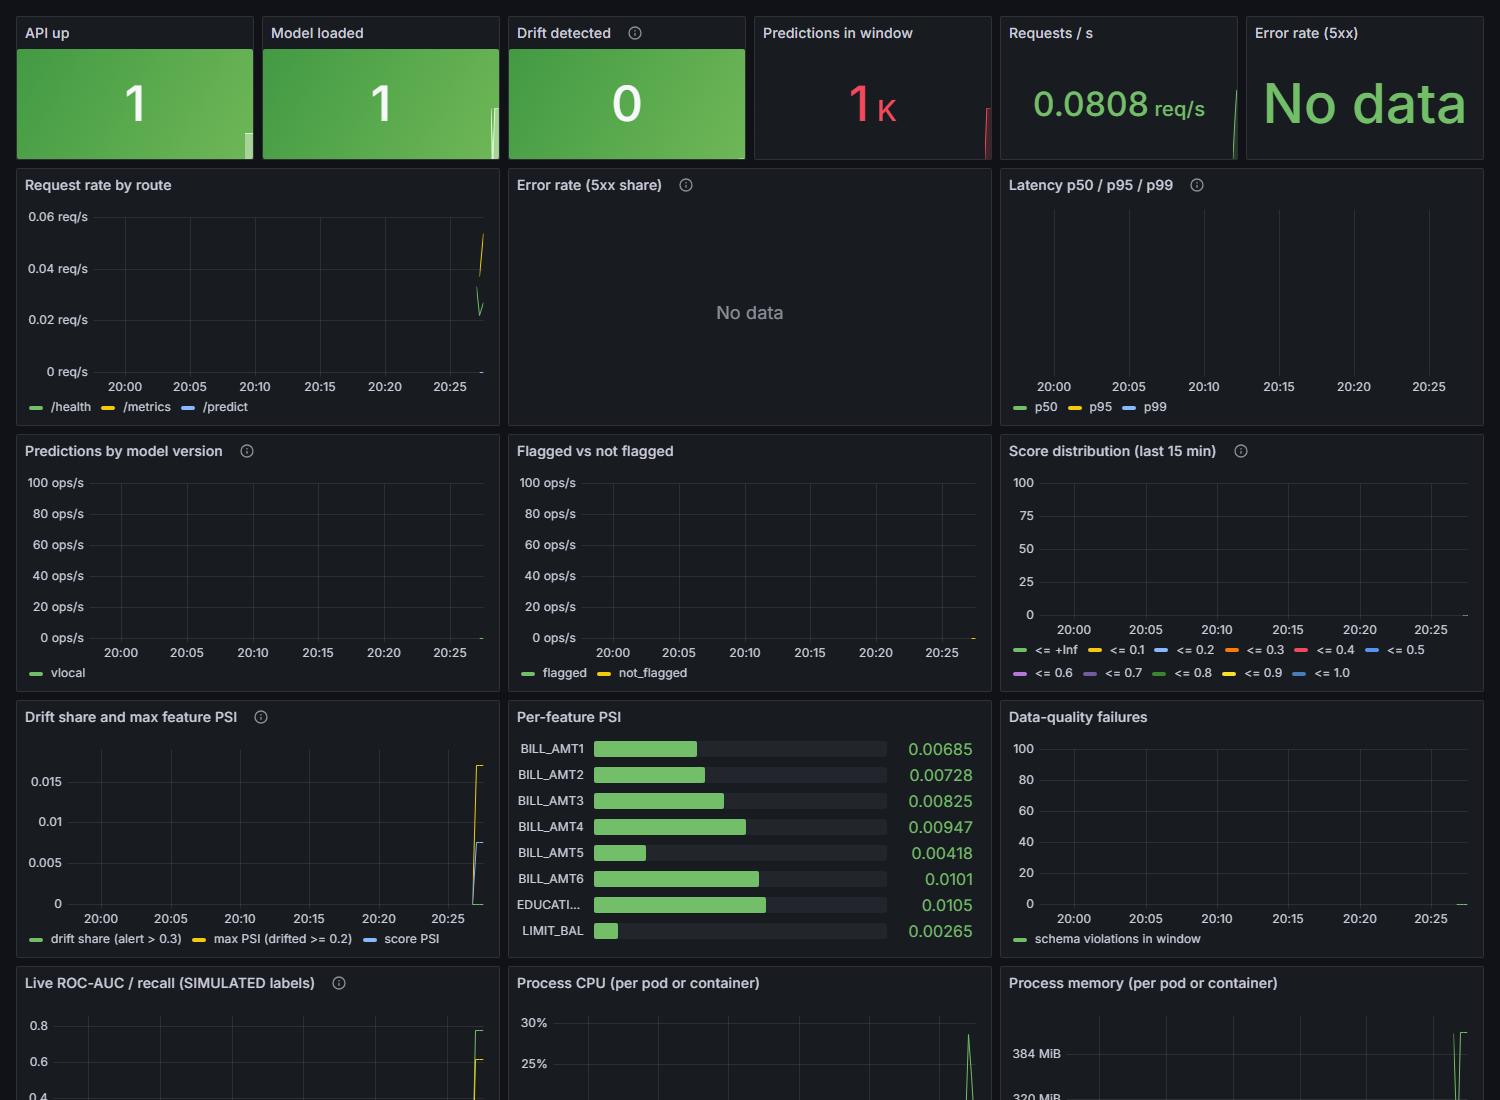
\includegraphics[width=\linewidth]{phase-8/01-normal-grafana.png}\caption{Normal traffic}\end{subfigure}\hfill
\begin{subfigure}{0.45\linewidth}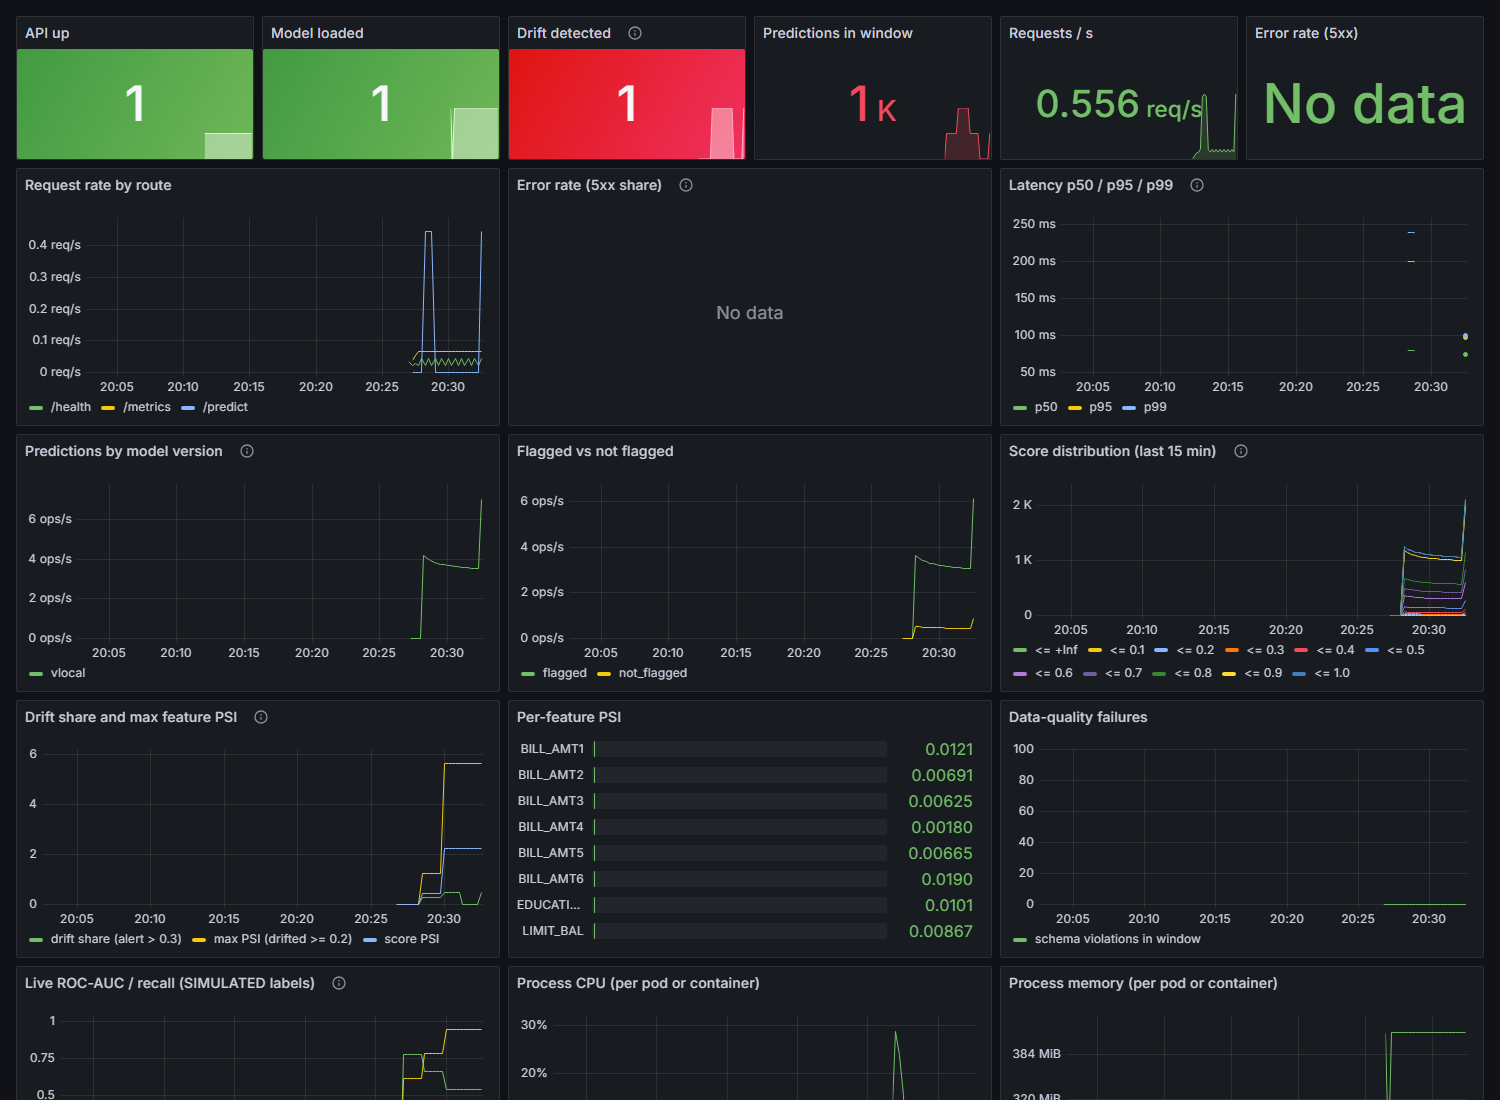
\includegraphics[width=\linewidth]{phase-8/02-degraded-grafana.png}\caption{Drifted traffic}\end{subfigure}\\[6pt]
\begin{subfigure}{0.45\linewidth}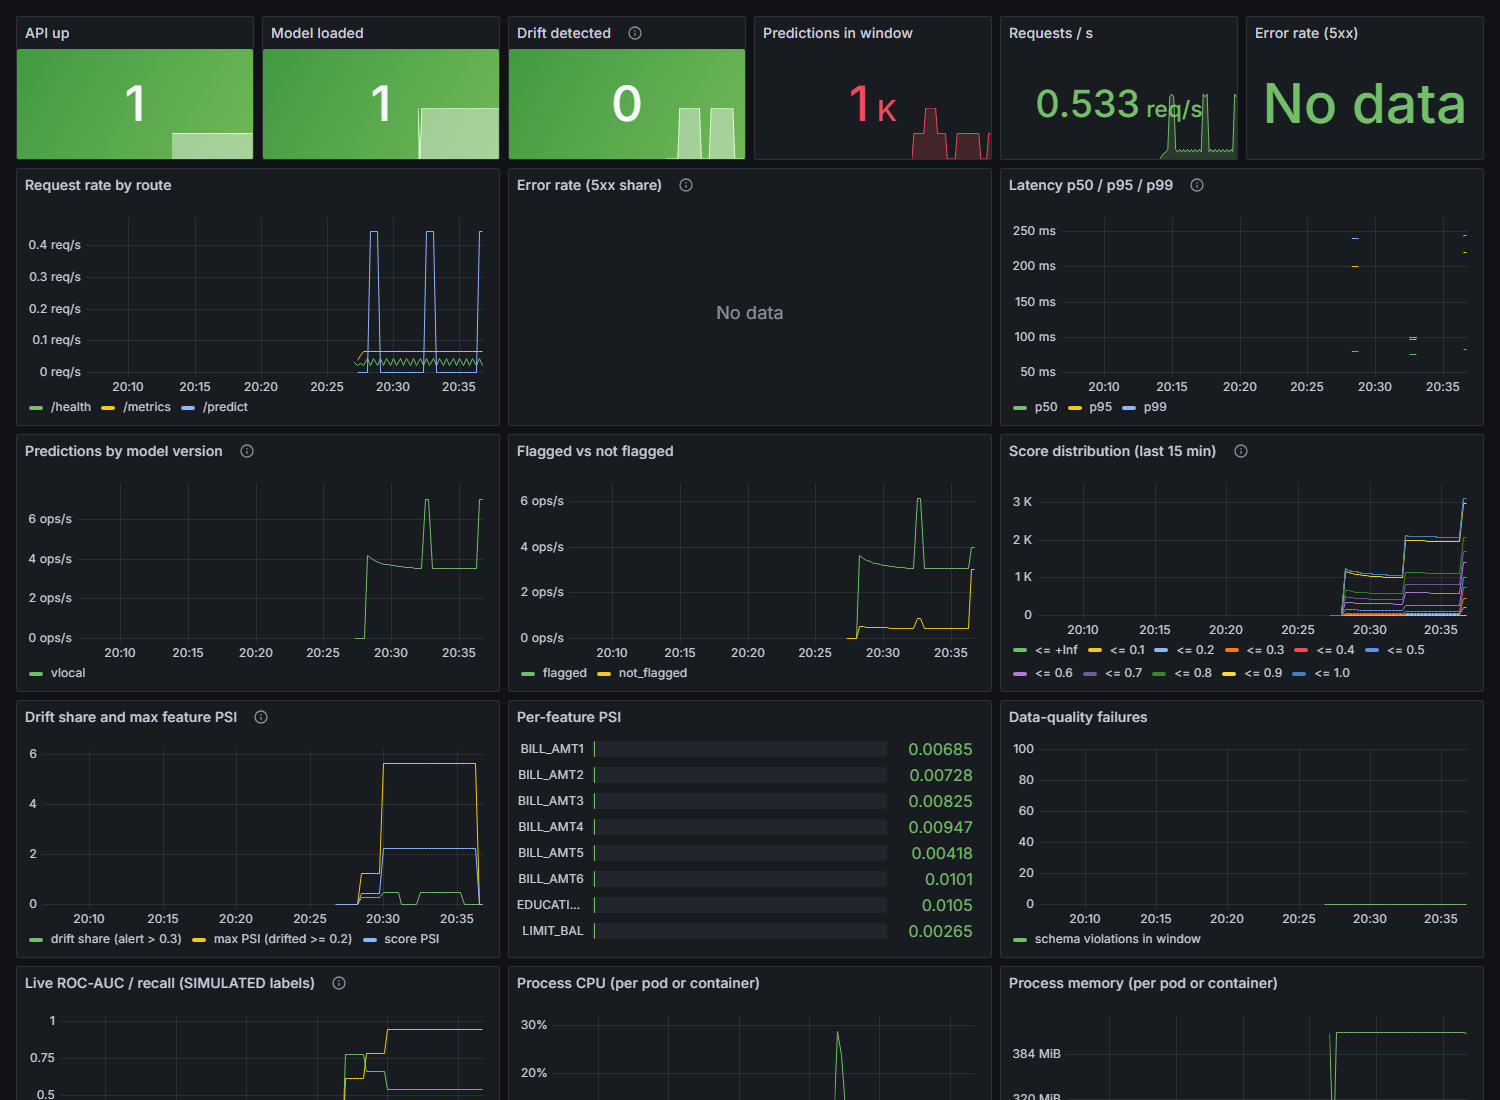
\includegraphics[width=\linewidth]{phase-8/04-resolved-grafana.png}\caption{Resolved after normal traffic returned}\end{subfigure}\hfill
\begin{subfigure}{0.45\linewidth}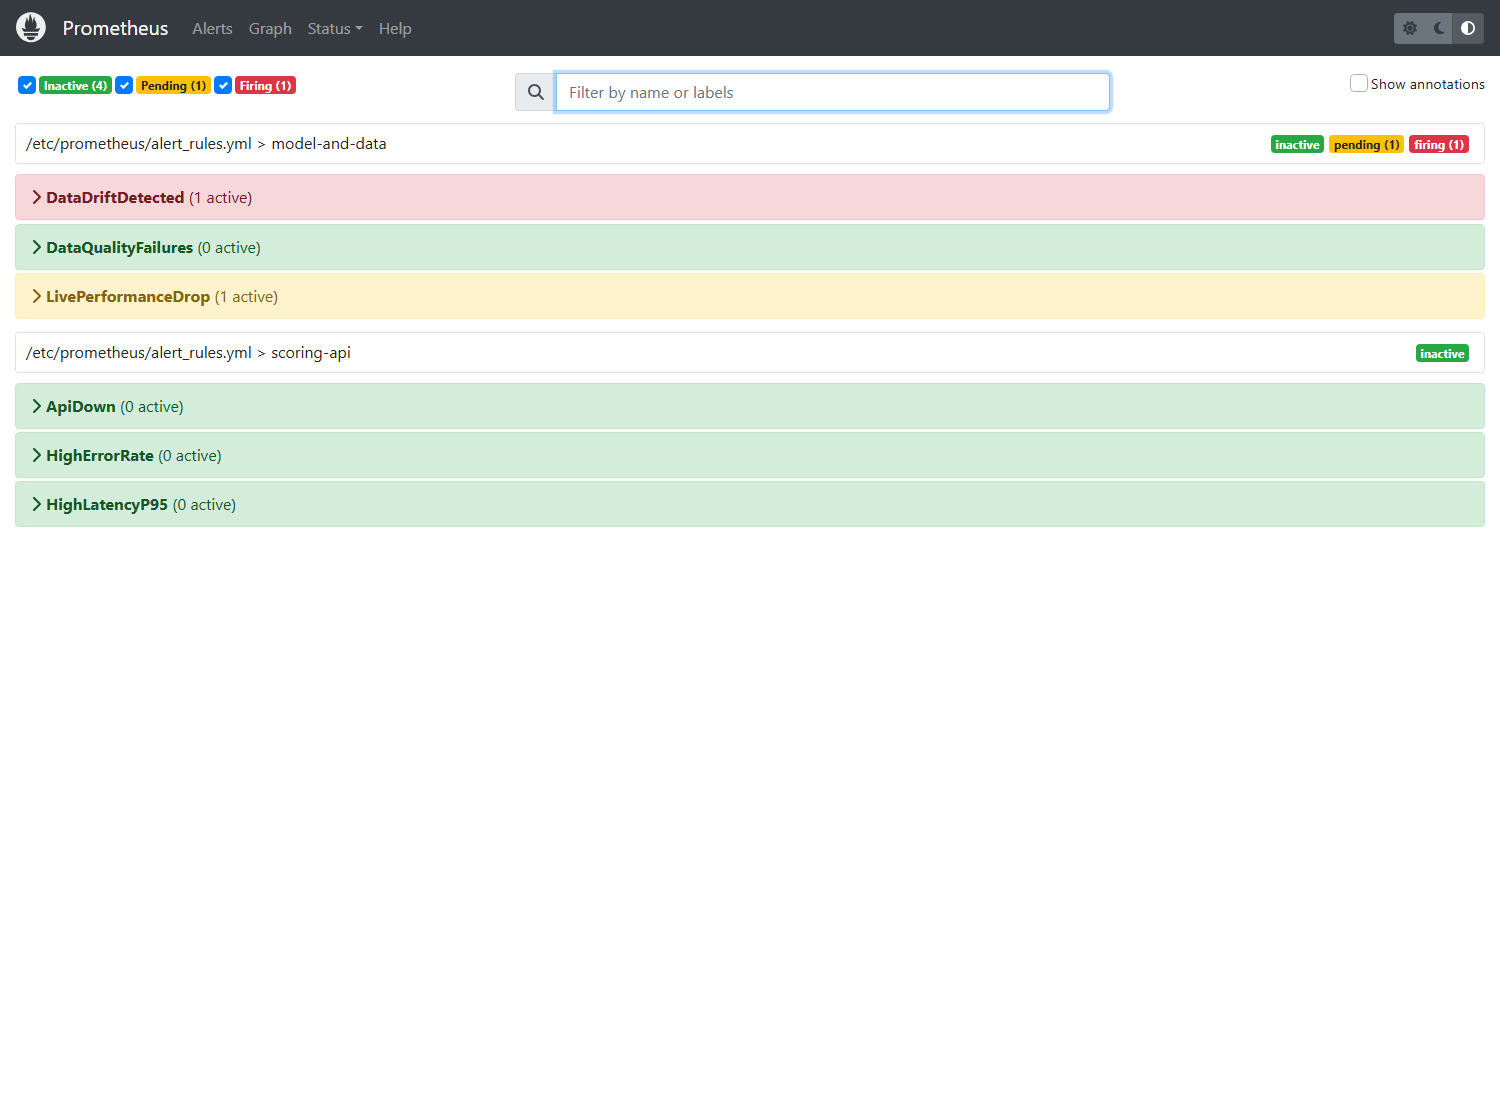
\includegraphics[width=\linewidth]{phase-8/03-alert-firing-prometheus-alerts.png}\caption{Prometheus: alert firing}\end{subfigure}
\caption{Grafana dashboard and alert states for the drift scenario (\simd{}).}
\end{figure}

\begin{table}[htbp]
\centering\small
\begin{tabularx}{\linewidth}{L{4.0cm}L{4.4cm}X}
\toprule
\hdr{Alert} & \hdr{How it was triggered} & \hdr{Fired $\rightarrow$ resolved (UTC, 2026-11-26)}\\
\midrule
\code{DataDriftDetected} & drifted traffic (1\,min \code{for}) & 15:31:18 $\rightarrow$ 15:31:48, then 15:33:48 $\rightarrow$ 15:35:48 (the window slid)\\
\code{HighErrorRate} (critical) & API restarted with a missing model (503) and about 148\,000 requests in 7\,min & 15:51:19 $\rightarrow$ 15:57:49\\
\code{HighLatencyP95} & 24 threads posting 100-record batches & 16:01:49 $\rightarrow$ 16:07:19\\
\code{LivePerformanceDrop} & live AUC under 0.70 on labelled drifted traffic & fired 15:49:18 (still firing: window lengthened to 1\,h for the retrain demo)\\
\bottomrule
\end{tabularx}
\caption{Alerts triggered on purpose. Every Alertmanager delivery is recorded with its time in \code{docs/evidence/phase-8/alert-notifications.log}.}
\end{table}

\begin{figure}[htbp]
\centering
\begin{subfigure}{0.45\linewidth}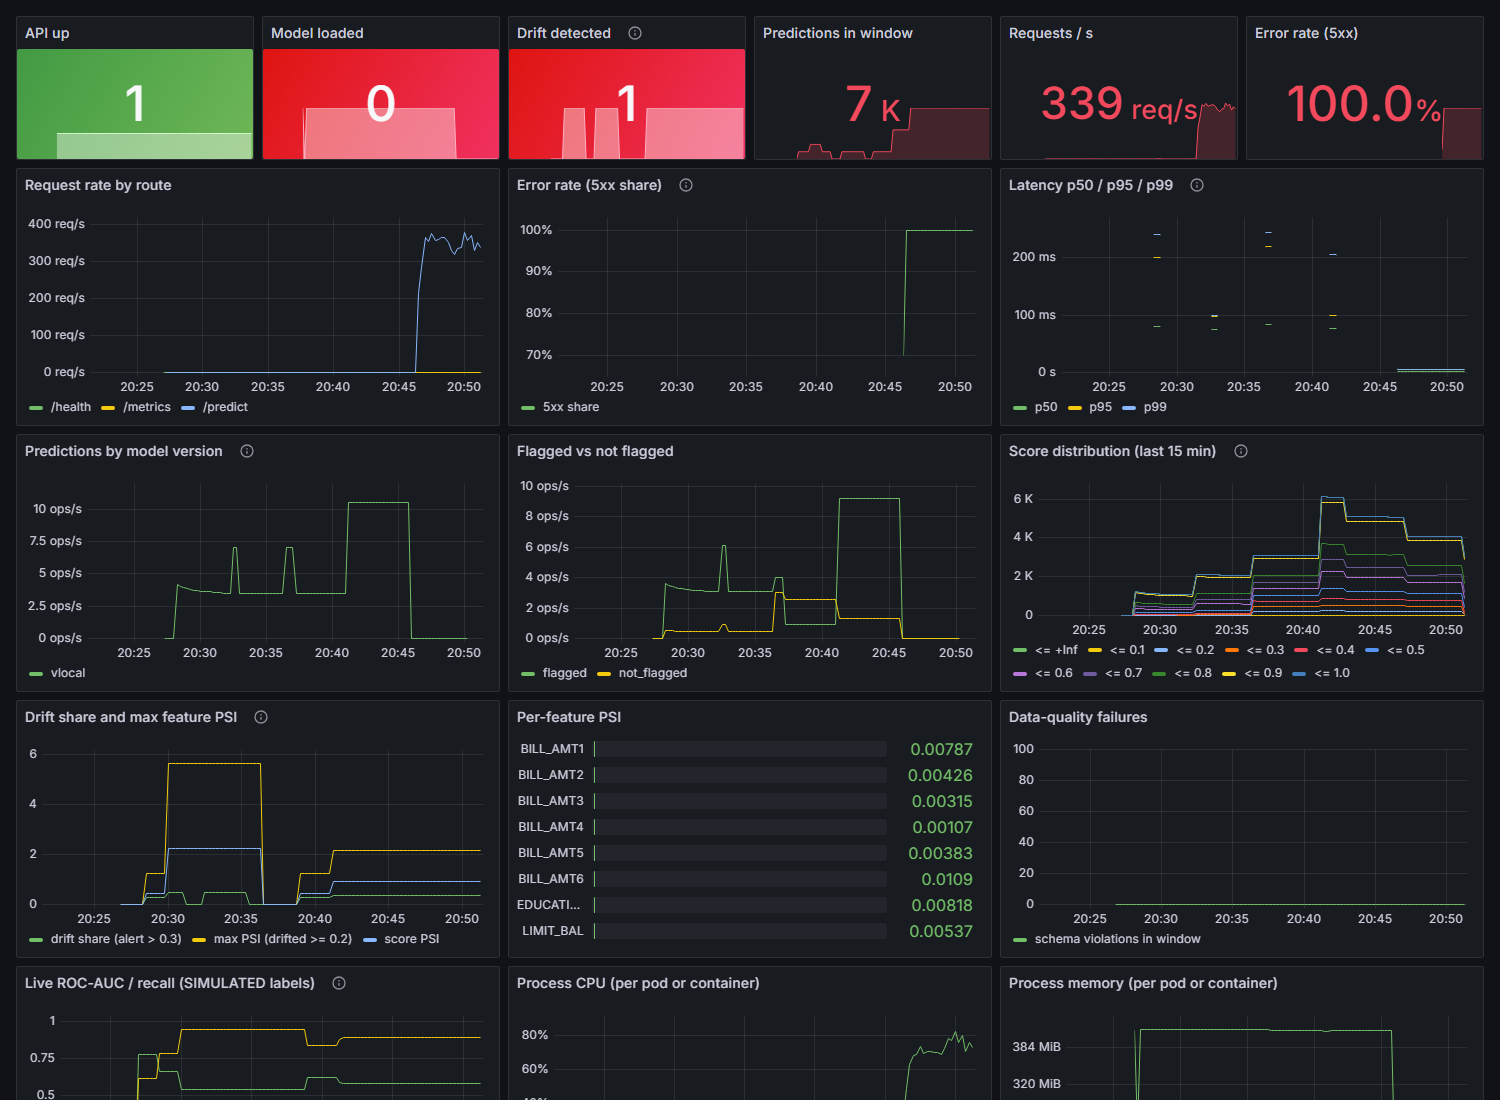
\includegraphics[width=\linewidth]{phase-8/05-error-rate-firing-grafana.png}\caption{Error rate firing}\end{subfigure}\hfill
\begin{subfigure}{0.45\linewidth}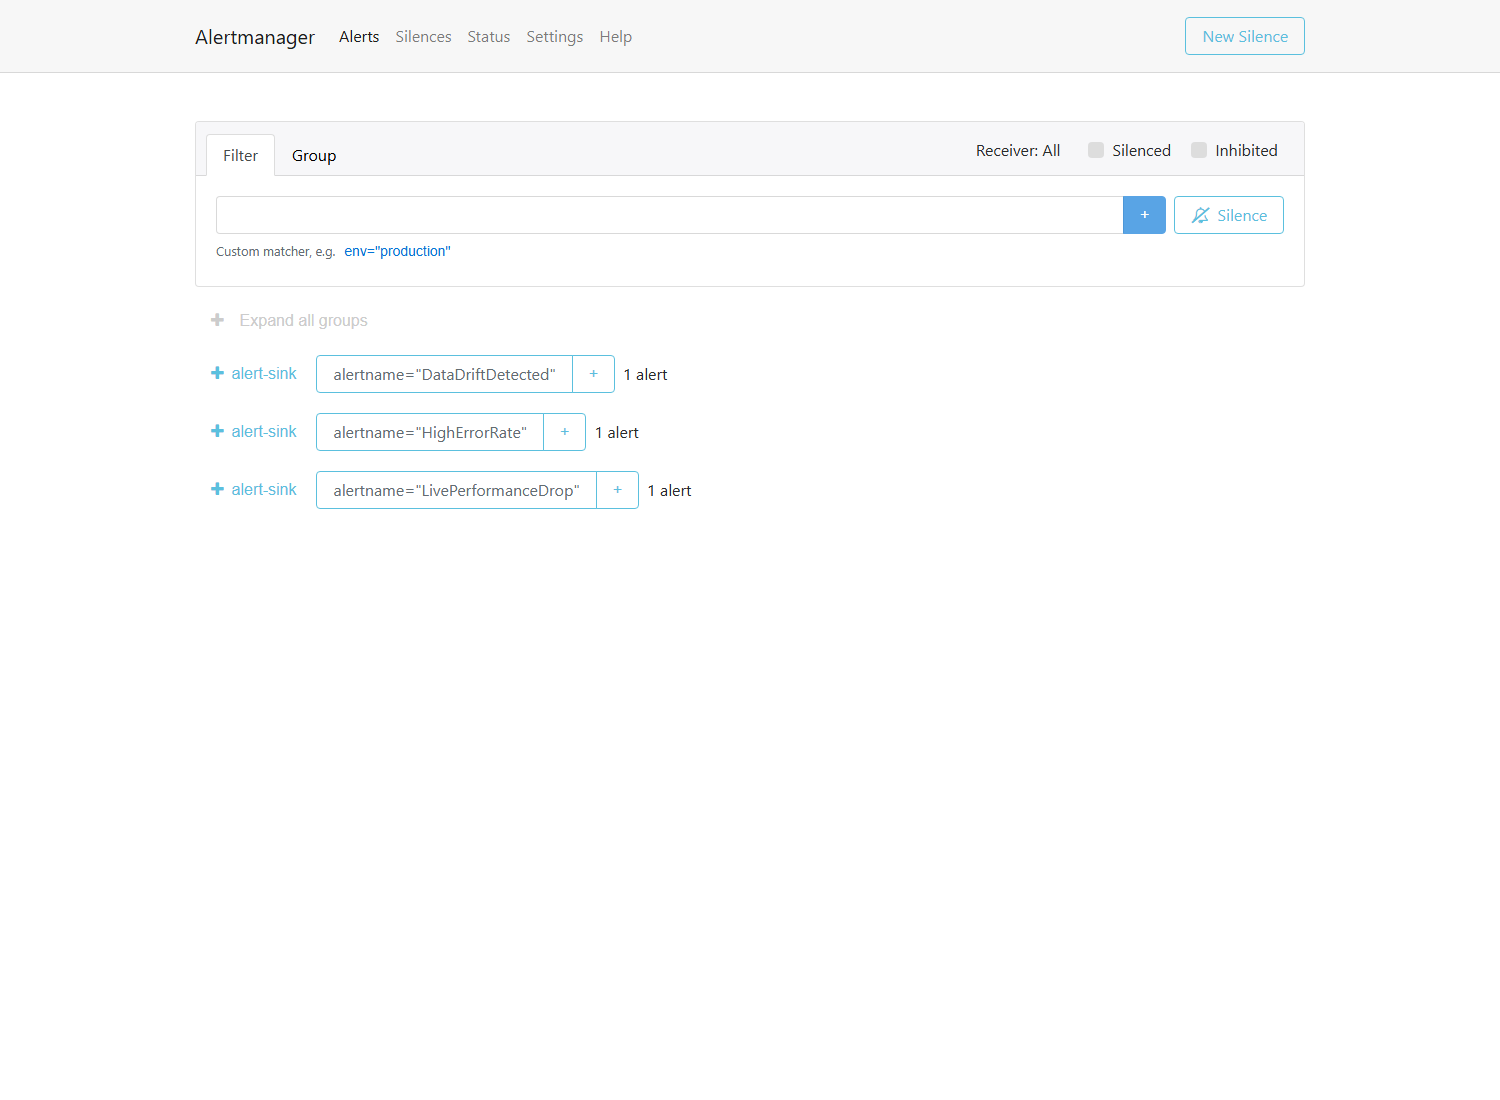
\includegraphics[width=\linewidth]{phase-8/05-error-rate-firing-alertmanager.png}\caption{Alertmanager: critical alert}\end{subfigure}\\[6pt]
\begin{subfigure}{0.45\linewidth}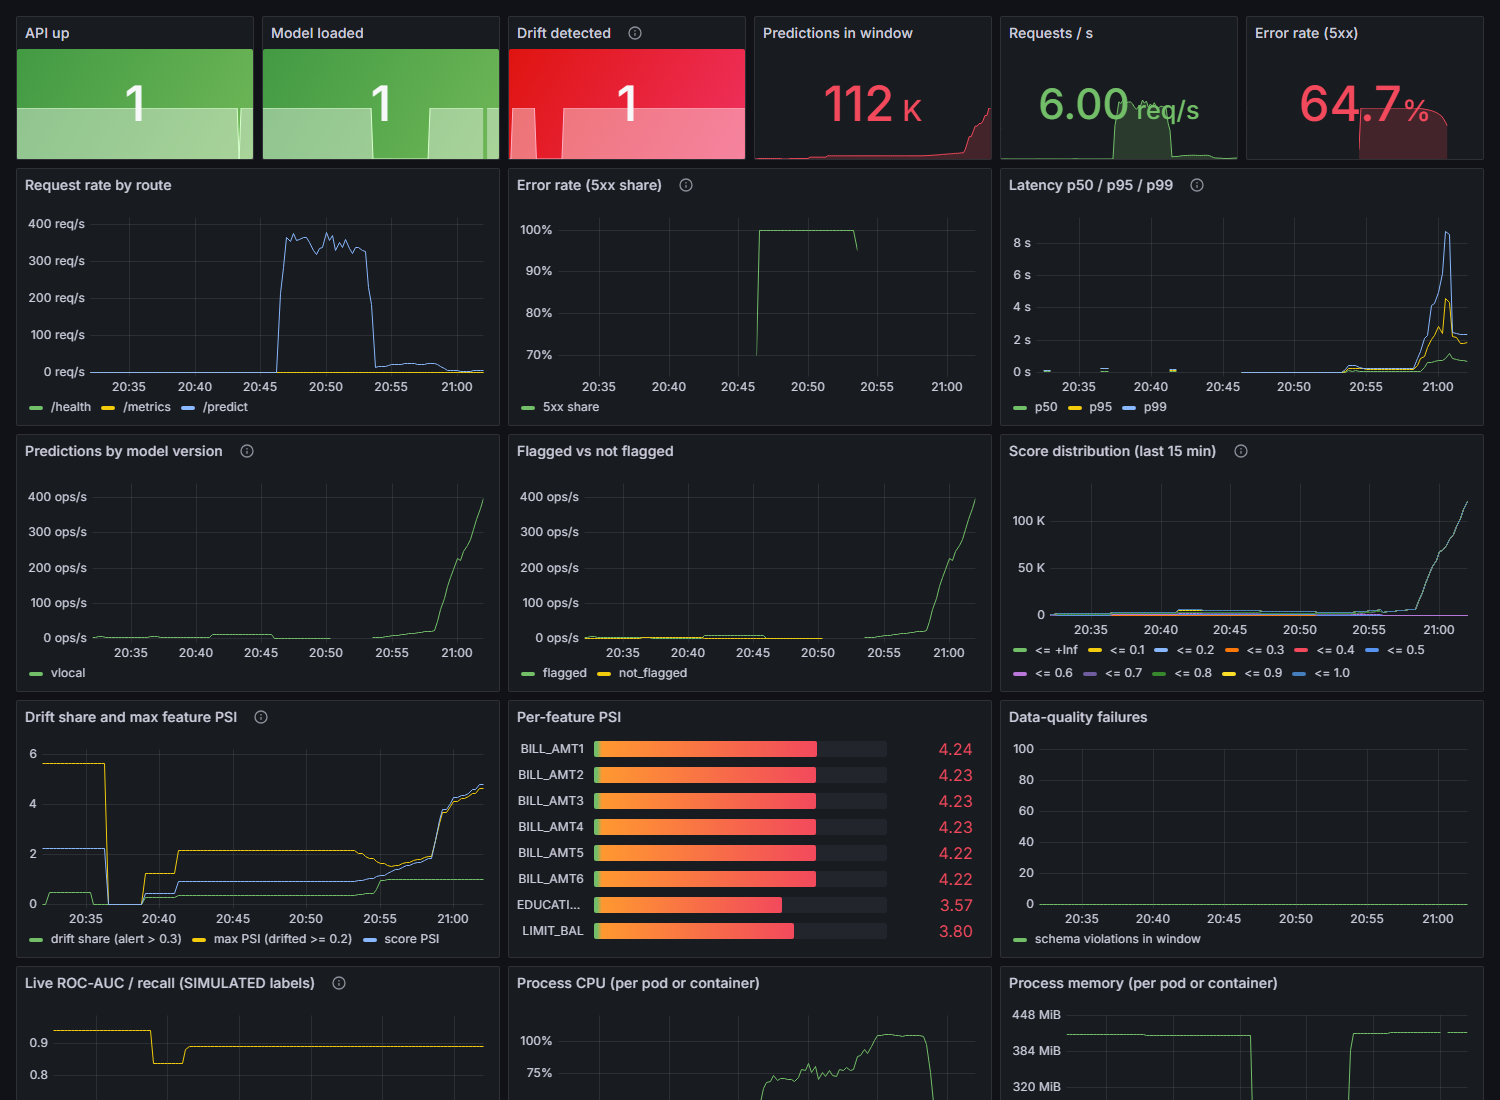
\includegraphics[width=\linewidth]{phase-8/06-latency-firing-grafana.png}\caption{p95 latency firing}\end{subfigure}\hfill
\begin{subfigure}{0.45\linewidth}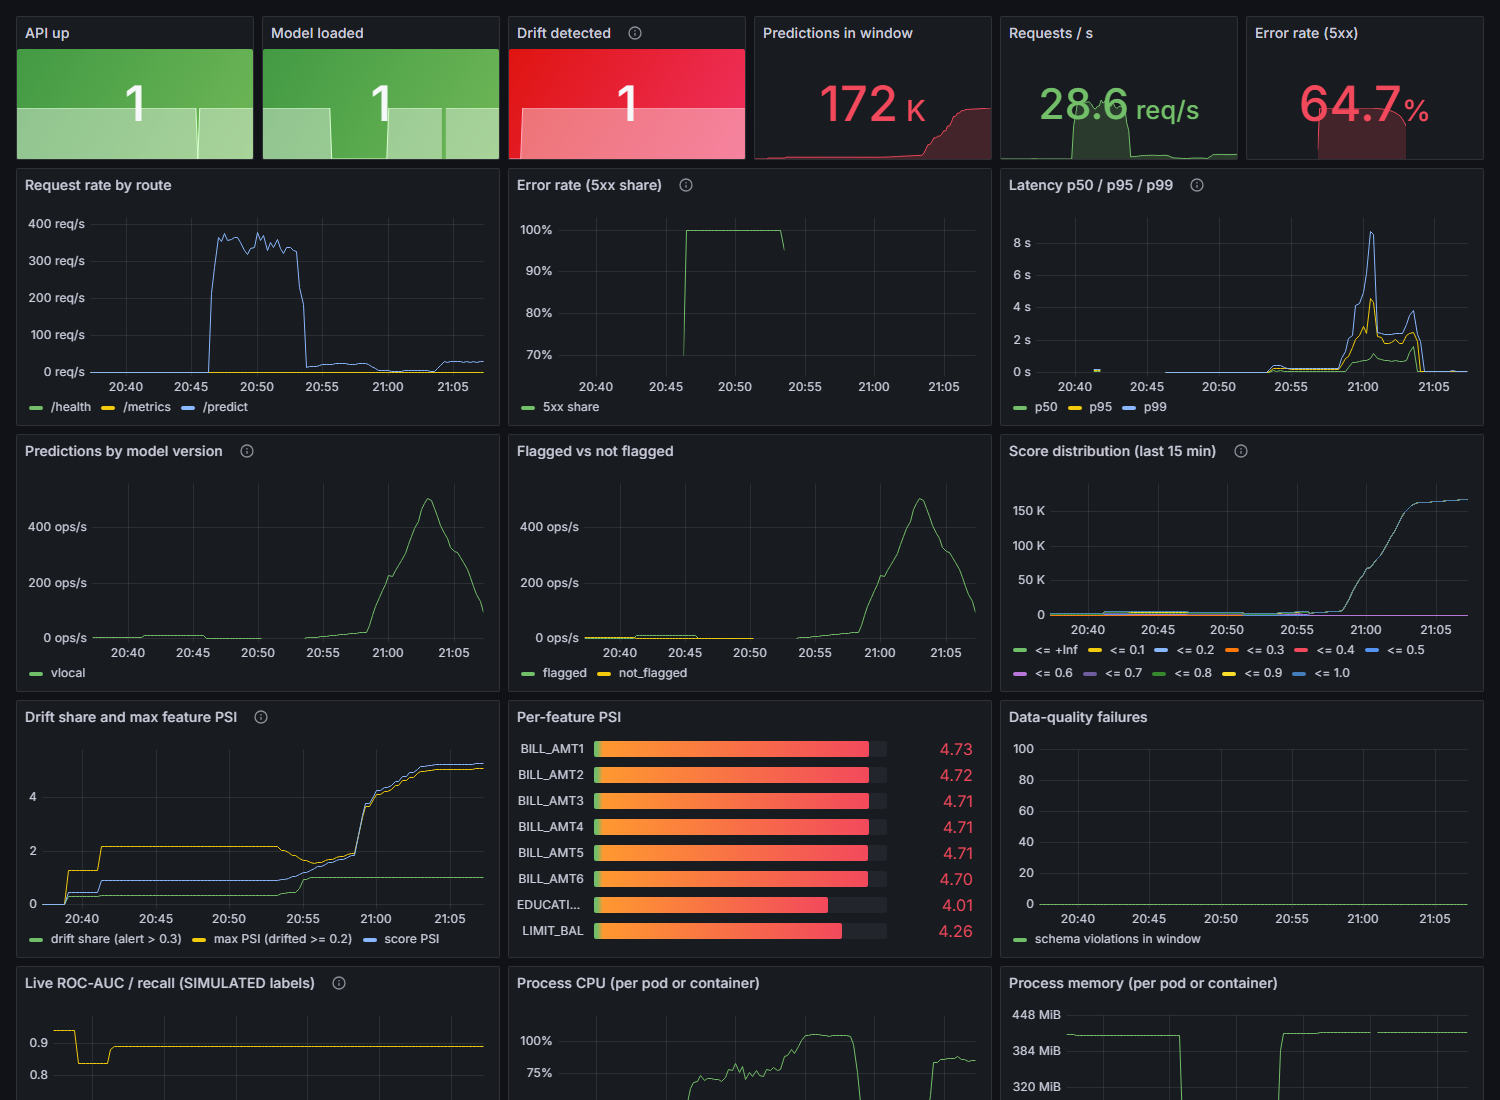
\includegraphics[width=\linewidth]{phase-8/06-latency-resolved-grafana.png}\caption{p95 latency resolved}\end{subfigure}
\caption{Error-rate and latency alerts.}
\end{figure}

\FloatBarrier
\subsection{Drift-triggered retraining}
\code{drift_watch_dag} checks the monitor every 10 minutes; on drift or a live-AUC drop (and no retrain in the last 6 hours) it starts \code{retrain_dag}, which re-runs the Phase 5 data tasks and Kubeflow run and then \emph{decides}: the challenger (alias \code{staging}) is compared with the champion on the test metrics MLflow recorded for each run (same seed and test size, which the step verifies) using predefined rules: ROC-AUC gain $\geq$ +0.005, PR-AUC and KS may drop by at most 0.01, and no fairness gap may grow by more than 0.02. The outcome is written to the model version; \emph{the DAG never moves the champion}, and a test asserts that no task calls the alias API.

\begin{table}[htbp]
\centering\small
\begin{tabularx}{\linewidth}{lRRR}
\toprule
\hdr{Metric (test)} & \hdr{Challenger v6} & \hdr{Champion v1} & \hdr{Rule}\\
\midrule
ROC-AUC & 0.7883 & 0.7883 & gain $\geq$ +0.005\\
PR-AUC & 0.5782 & 0.5782 & drop $\leq$ 0.01\\
KS & 0.4401 & 0.4401 & drop $\leq$ 0.01\\
\midrule
\multicolumn{4}{l}{ROC-AUC gain: $+0.0000$ \quad\textbf{Decision: rejected} (below the required $+0.0050$)}\\
\bottomrule
\end{tabularx}
\caption{The live drift-triggered run \code{retrain-drift-acceptance} (\simd{} drift). Retraining on unchanged data reproduces the champion exactly, so the rejection path was exercised; the champion stayed on v1.}
\end{table}

What this shows: the trigger chain, the same-holdout comparison, the rejection rule, and that nothing is promoted automatically. What it does \emph{not} show: a better challenger being recommended, approved and promoted through the Deploy workflow (unit-tested only), and a fairness re-evaluation inside the DAG (the test split lives in the Kubeflow pods; the decision says so and tells the approver to check \code{reports/fairness.json}). Problems found by running it: a duplicate-DAG error from importing one DAG file into another, a first decision step with no test split, a watcher that re-triggered every ten minutes (now a 6-hour cooldown), and a rerun that could not find its own training run after a task was cleared (re-run the DAG instead).

\subsection{Promotion and rollback}
Promotion is a run of the Deploy workflow with a model version, approved by the required reviewer: check that the version was recommended or is a former champion, fetch its files from the registry archive, build, scan, deploy, smoke-test, and only then move \code{champion} (tagging the old model for rollback). A failed deployment never touches the alias, so \code{champion} always names a model that is serving. Rollback is the same workflow with the previous champion's version, the Rollback workflow (\code{previous}, a revision or a SHA), or \code{kubectl rollout undo} locally.

% =====================================================================================================
\section{Security, ethics and risk}
\label{sec:security}

\subsection{Scans and controls}
\begin{table}[htbp]
\centering\small
\begin{tabularx}{\linewidth}{L{2.7cm}L{4.3cm}X}
\toprule
\hdr{Tool} & \hdr{Scope} & \hdr{Result}\\
\midrule
gitleaks & full history (42 commits) & no leaks\\
bandit & \code{src/} (4\,714 lines) & 0 medium, 0 high, 3 low (informational)\\
pip-audit & locked dependencies & no known vulnerabilities; one accepted, documented risk (\code{diskcache}, no fixed version, not reachable)\\
Trivy & API, monitor and frontend images & 0 HIGH/CRITICAL with a fix, each\\
\bottomrule
\end{tabularx}
\caption{Security scan results (2026-11-26).}
\end{table}
Other controls: pre-commit and CI secret scanning; secrets from Secrets Manager or the environment, never git; OIDC instead of AWS keys; least-privilege IAM scoped to single resources; non-root containers with build tools removed from runtime images; API key (40 random characters, constant-time comparison) on every business endpoint; request size and batch limits; per-client rate limiting (600 requests/minute); no personal data in application logs; GitHub Actions pinned to commit SHAs.

\subsection{Ethics and limits}
The data reflects one country and one bank in 2005 and carries gender, age and marital-status patterns. Sensitive attributes are excluded from the inputs but proxy effects remain (Section~\ref{sec:fairness}); the model card states intended use, limitations and fairness findings. The output is a ranking score and every interface says the system is not a lending tool.

\subsection{Risk assessment}
\begin{longtable}{L{0.8cm}L{5.0cm}L{0.9cm}L{0.9cm}L{6.0cm}}
\toprule
\hdr{\#} & \hdr{Risk} & \hdr{L} & \hdr{I} & \hdr{Main mitigation}\\
\midrule\endhead
R1 & unfair outcomes across groups & H & H & sensitive attributes not inputs; per-group metrics; challenger may not widen gaps\\
R2 & score read as a probability or used for real decisions & H & H & score named \code{risk_score} (type \code{uncalibrated_risk_score}), disclaimers, bands not percentages\\
R3 & silent data drift & M & H & drift monitor, alerts, retrain watcher, human-approved promotion\\
R4 & credential leak & M & H & gitleaks (hook and CI), secrets outside git, OIDC\\
R5 & cloud cost overrun, forgotten resources & M & M & smallest sizes, no NAT or load balancer, two stacks, teardown script with leftover list\\
R6 & public endpoint abuse, eavesdropping & M & M & one-CIDR API, key, size and rate limits (UI port open only for the demo; HTTP only)\\
R7 & bad model or image reaches production & M & H & CI gates, quality gate in CD, reviewer approval, smoke test, rollback\\
R8 & overclaiming simulated results & M & M & everything simulated is labelled in docs, scripts and dashboards\\
R9 & supply-chain compromise & L & H & pinned dependencies and actions, pip-audit, Trivy\\
R10 & personal data in monitoring data & L & M & pseudonymised log, 30-day retention, separate from app logs\\
R11 & single point of failure & M & L & accepted for coursework; ECS replaces a failed task; Kubernetes demo shows replicas\\
\bottomrule
\end{longtable}
\textit{L = likelihood, I = impact.} Open risks: a single-person approval gate, an unconfirmed hard AWS spend limit, and the public UI port, which holds the API key server-side and is therefore only acceptable for a short demonstration.

% =====================================================================================================
\section{Automation versus manual steps}
\begin{table}[htbp]
\centering\small
\begin{tabularx}{\linewidth}{L{5.2cm}L{3.2cm}X}
\toprule
\hdr{Step} & \hdr{Automated} & \hdr{Manual gate}\\
\midrule
Lint, tests, scanners, image build and scan on every push & yes & merge needs a review and green CI\\
Data fetch, validation, DVC publication, training, evaluation, registration & yes (one Airflow trigger) & none\\
Quality gate & yes & none; it cannot be waived\\
Drift detection and retrain trigger & yes & none\\
Challenger versus champion decision & yes (predefined rules) & accepting a challenger is a human act\\
Promotion and deployment to production & the workflow does the work & required reviewer approves the \code{production} environment\\
Rollback & automatic on a failed smoke test & manual rollback or re-promotion\\
AWS teardown & one script & someone must run it and check the console\\
\bottomrule
\end{tabularx}
\caption{What is automated and where a human decides.}
\end{table}

% =====================================================================================================
\section{Reproduction and clean-up}
\label{sec:cleanup}

\textbf{Reproduce.} The README gives the ordered steps: clone, create the environment, \code{dvc pull}, \code{dvc repro}, run the tests, start the Compose stack, run the drift scenario, and deploy. A copy of the configuration names (no values) for GitHub, AWS, DagsHub and MLflow is in the README table \emph{Configuration names}; values live only in \code{.env}, \code{.dvc/config.local}, GitHub settings and Secrets Manager. A reproduction by someone who did not write the README is still required (Section~\ref{sec:summary}).

\textbf{Clean-up after the demonstration.} Billable AWS resources are removed unless hosting is explicitly approved: run \code{./infra/aws/teardown.sh --yes}; check that the list of stacks, clusters, ECR repositories, secrets and log groups is empty (the only expected leftover is the pre-existing DVC bucket); check the console for Elastic IPs and network interfaces; check Cost Explorer the next day; confirm that the old addresses no longer answer; then stop the local Docker, Airflow and Minikube stacks. The numbered steps are in the README section \emph{Clean up}.

% =====================================================================================================
\section{Lessons learned}
\begin{itemize}
\item \textbf{Run it for real.} Almost every real bug appeared only in a live run: a request-id collision on a shared server, retries of non-retryable failures, Windows quoting that broke \code{kubectl}, a self-healing demo that deleted a pod already terminating, a watcher that re-triggered every ten minutes, and on AWS an OIDC subject format that no documentation had warned about.
\item \textbf{Make deterministic outcomes first-class.} An exit-code contract (validation 2, gate 3) turned wasted retries into immediate, readable failures.
\item \textbf{Evidence beats claims.} Where something was not run (the autoscaler, a better-than-champion challenger, the AWS rollback), the documents say so.
\item \textbf{Cost and safety are design inputs.} No load balancer or NAT gateway, IAM scoped to single resources, and teardown as a stack deletion.
\item \textbf{Preview infrastructure changes.} Reading the CloudFormation change set before executing it avoided resetting the running service.
\item \textbf{Simulated data needs a label.} A convincing dashboard is easily mistaken for field evidence.
\end{itemize}

% =====================================================================================================
\section{Individual contributions}
\label{sec:contrib}
Contributions are taken from the Git history and the ownership map in \code{.github/CODEOWNERS}. \textbf{Each member should confirm or amend this table before submission.}

\begin{longtable}{L{3.2cm}L{11.4cm}}
\toprule
\hdr{Member} & \hdr{Contribution}\\
\midrule\endhead
S2 -- Hashir Rauf (\texttt{@Hashir-Rauf}) & Repository governance and CI/CD; data ingestion and validation; Flask API, Docker images, Compose stacks and the Next.js interface; Airflow acceptance runs and fixes; AWS infrastructure, deploy and rollback workflows and the live deployment; Kubernetes manifests and demo; monitoring, prediction log, drift monitor, retrain DAG and promotion workflow; security audit, risk assessment and documentation\\
S1 -- Junaid Minhas (\texttt{@JA-Codex}) & Modelling: features, Feast, tuning, training, evaluation, fairness, explanations, simulated drift scenarios and the promotion rules (\code{src/features}, \code{src/models}, \code{src/common}, \code{configs}, \code{feature_repo}, notebooks and the modelling tests). Phase 5 (Airflow and Kubeflow) was merged through a pull request and then verified and fixed in the acceptance runs\\
S3 -- Ahsan Ijaz & \\
\bottomrule
\end{longtable}
An AI coding assistant helped with parts of the implementation; it authored no commit. All commits are made under the team members' own identities, as the project rules require.

% =====================================================================================================
\appendix
\section{Evidence index}
All evidence lives in the repository under \code{docs/evidence/}. Figures in this report are included directly from those folders.

\begin{longtable}{L{2.6cm}L{12.0cm}}
\toprule
\hdr{Folder} & \hdr{Contents}\\
\midrule\endhead
\code{phase-0} & pre-commit blocks a secret (log)\\
\code{phase-1} & DVC reproduction demo, remotes in sync, corrupt-versus-good validation, merge-conflict exercise, DagsHub view\\
\code{phase-2} & first and repeated training metrics, Feast online sample, fairness and registration reports\\
\code{phase-3} & CI red and green runs, independent audit of the modelling work, scanner results\\
\code{phase-4} & API curl transcript, stack check, BentoML run, interface screenshots\\
\code{phase-5} & acceptance runs, Airflow and Kubeflow screenshots, problems found and fixed\\
\code{phase-6} & live AWS evidence and screenshots of the deployed interface\\
\code{phase-7} & Kubernetes demo log and summary\\
\code{phase-8} & Grafana, Prometheus and Alertmanager screenshots, alert notification log, retrain run and decision\\
\code{phase-9} & gitleaks, bandit, pip-audit and Trivy outputs\\
\bottomrule
\end{longtable}

\end{document}
